%%%%%%%%%%%%%%%%%%%%%%%%%%%%%%%%%%%%%%%%%
% Minimalist Book Title Page
% LaTeX Template
% Version 2.0 (21/7/17)
%
% This template was downloaded from:
% http://www.LaTeXTemplates.com
%
% Original author:
% Peter Wilson (herries.press@earthlink.net) with modifications by:
% Vel (vel@latextemplates.com)
%
% License:
% CC BY-NC-SA 3.0 (http://creativecommons.org/licenses/by-nc-sa/3.0/)
%
%%%%%%%%%%%%%%%%%%%%%%%%%%%%%%%%%%%%%%%%%

%---------------------------------------------------------------------------------
%	PACKAGES AND OTHER DOCUMENT CONFIGURATIONS
%---------------------------------------------------------------------------------

\documentclass[a4paper, 11pt,openany]{book} % A4 paper size and default 11pt font size

\usepackage[svgnames]{xcolor} % Required for colour specification
\usepackage[utf8]{inputenc} % Required for inputting international characters
\usepackage[T1]{fontenc} % Output font encoding for international characters
\usepackage{PTSerif} % Use the Paratype Serif font

\usepackage{graphicx,float} %graphic management system
\graphicspath{ {./images/} }
\usepackage{mathtools}
\usepackage{tikz}

\usepackage{geometry}
\geometry{margin=1in}

\usepackage{indentfirst}

\usepackage{enumitem}

\usepackage{listings}
\usepackage{color}

\colorlet{punct}{red!60!black}
\definecolor{background}{HTML}{EEEEEE}
\definecolor{delim}{RGB}{20,105,176}
\colorlet{numb}{magenta!60!black}
 
\definecolor{codegreen}{rgb}{0,0.6,0}
\definecolor{codegray}{rgb}{0.5,0.5,0.5}
\definecolor{codepurple}{rgb}{0.58,0,0.82}
\definecolor{backcolour}{rgb}{0.95,0.95,0.92}
\definecolor{vgucolor}{rgb}{0.99,0.50,0.27}
\usepackage{graphicx,float} %graphic management system
\graphicspath{ {./images/} }
\usepackage[
backend=biber,
style=numeric,
sorting=none
]{biblatex}
\usepackage{tikz}
\usetikzlibrary{arrows,automata}
\usepackage{amsmath}
\usepackage{amssymb}
\setlength{\parindent}{0cm}
\setlength{\parskip}{0.75em}
%%
\usepackage{ifthen}
\usepackage[a4paper, total={6in, 8in}]{geometry}
\usepackage{url}
\usepackage{listings}

%% caption less table to specify restful primitives
\newcommand{\restful}[1]
{
\begin{center}
\begin{tabular}{l p{12cm}}
\hline
#1
\hline
\end{tabular}
\end{center}
\vspace{6pt}
}


%% caption less table to specify restful uri
\newcommand{\routes}[1]
{
\begin{center}
\begin{tabular}{p{\textwidth}}
\hline
#1
\hline
\end{tabular}
\end{center}
\vspace{6pt}
}
%
%
%
  
\newcommand{\mimetype}[2]{#1 & #2 \\\noalign{\smallskip}}
\newcommand{\head}[2]{#1 & #2 \\\noalign{\smallskip}}
\newcommand{\uri}[2]{\url{#1} \\ #2 \vspace{8pt} \\\noalign{\smallskip}}
\newcommand{\env}[2]{#1 & #2 \\\noalign{\smallskip}}
%

%%% resource definition table
\newcommand{\resource}[1]
{
\begin{center}
\begin{tabular}{l l p{12cm}}
\hline
#1
\hline
\end{tabular}
\end{center}
\vspace{6pt}
}
\newcommand{\attr}[3]{{\tt #1} & #2 & #3 \\\noalign{\smallskip}}

%
%
\newcommand{\request}[6]
{
\begin{center}
\begin{tabular}{l p{12cm}}
\hline
Synopsis:  & #1 \url{#2} \\\noalign{\smallskip}
           & #3     \vspace{4pt}\\ 
Precondition:  & #4 \vspace{4pt}\\
Postcondition: & #5 \vspace{4pt}\\
Status code:   & #6 \\
\hline
\end{tabular}
\end{center}
\vspace{6pt}
}

\newcommand{\sep}{\\\noalign{\smallskip} &}

\newcommand{\status}[1]
{
\ifthenelse{\equal{#1}{100}}{100 Continue}{}%
\ifthenelse{\equal{#1}{101}}{101 Switching Protocols}{}%
\ifthenelse{\equal{#1}{200}}{200 OK}{}%
\ifthenelse{\equal{#1}{201}}{201 Created}{}%
\ifthenelse{\equal{#1}{202}}{202 Accepted}{}%
\ifthenelse{\equal{#1}{203}}{203 Non-Authoritative Information}{}%
\ifthenelse{\equal{#1}{204}}{204 No Content}{}%
\ifthenelse{\equal{#1}{205}}{205 Reset Content}{}%
\ifthenelse{\equal{#1}{206}}{206 Partial Content}{}%
\ifthenelse{\equal{#1}{300}}{300 Multiple Choices}{}%
\ifthenelse{\equal{#1}{301}}{301 Moved Permanently}{}%
\ifthenelse{\equal{#1}{302}}{302 Found}{}%
\ifthenelse{\equal{#1}{303}}{303 See Other}{}%
\ifthenelse{\equal{#1}{304}}{304 Not Modified}{}%
\ifthenelse{\equal{#1}{307}}{307 Temporary Redirect}{}%
\ifthenelse{\equal{#1}{302}}{302 Found}{}%
\ifthenelse{\equal{#1}{400}}{400 Bad Request}{}%
\ifthenelse{\equal{#1}{401}}{401 Unauthorized}{}%
\ifthenelse{\equal{#1}{402}}{402 Payment Required}{}%
\ifthenelse{\equal{#1}{403}}{403 Forbidden}{}%
\ifthenelse{\equal{#1}{404}}{404 Not Found}{}%
\ifthenelse{\equal{#1}{405}}{405 Method Not Allowed}{}%
\ifthenelse{\equal{#1}{406}}{406 Not Acceptable}{}%
\ifthenelse{\equal{#1}{407}}{407 Proxy Authentication Required}{}%
\ifthenelse{\equal{#1}{408}}{408 Request Timeout}{}%
\ifthenelse{\equal{#1}{409}}{409 Conflict}{}%
\ifthenelse{\equal{#1}{410}}{410 Gone}{}%
\ifthenelse{\equal{#1}{411}}{411 Length Required}{}%
\ifthenelse{\equal{#1}{412}}{412 Precondition Failed}{}%
\ifthenelse{\equal{#1}{413}}{413 Request Entity Too Large}{}%
\ifthenelse{\equal{#1}{414}}{414 Request-URI Too Long}{}%
\ifthenelse{\equal{#1}{415}}{415 Unsupported Media Type}{}%
\ifthenelse{\equal{#1}{416}}{416 Requested Range Not Satisfiable}{}%
\ifthenelse{\equal{#1}{417}}{417 Expectation Failed}{}%
\ifthenelse{\equal{#1}{422}}{422 Unprocessable Entity}{}%
\ifthenelse{\equal{#1}{500}}{500 Internal Server Error}{}%
\ifthenelse{\equal{#1}{501}}{501 Not Implemented}{}%
\ifthenelse{\equal{#1}{502}}{502 Bad Gateway}{}%
\ifthenelse{\equal{#1}{503}}{503 Service Unavailable}{}%
\ifthenelse{\equal{#1}{504}}{504 Gateway Timeout}{}%
\ifthenelse{\equal{#1}{505}}{505 HTTP Version Not Supported}{}%
}

\newcommand{\httpcode}[2]{\status{#1} & #2 \\\noalign{\smallskip}}

\newcommand{\example}[1]{\noindent {\bf #1}}
\addbibresource{references.bib}
 
\lstdefinestyle{customc}{
  belowcaptionskip=1\baselineskip,
  breaklines=true,
  frame=L,
  xleftmargin=\parindent,
  language=C,
  showstringspaces=false,
  basicstyle=\footnotesize\ttfamily,
  keywordstyle=\bfseries\color{green!40!black},
  commentstyle=\itshape\color{purple!40!black},
  identifierstyle=\color{blue},
  stringstyle=\color{orange},
}

\lstdefinelanguage{json}{
    basicstyle=\normalfont\ttfamily,
    numbers=left,
    numberstyle=\scriptsize,
    stepnumber=1,
    numbersep=8pt,
    showstringspaces=false,
    breaklines=true,
    frame=lines,
    backgroundcolor=\color{background},
    literate=
     *{0}{{{\color{numb}0}}}{1}
      {1}{{{\color{numb}1}}}{1}
      {2}{{{\color{numb}2}}}{1}
      {3}{{{\color{numb}3}}}{1}
      {4}{{{\color{numb}4}}}{1}
      {5}{{{\color{numb}5}}}{1}
      {6}{{{\color{numb}6}}}{1}
      {7}{{{\color{numb}7}}}{1}
      {8}{{{\color{numb}8}}}{1}
      {9}{{{\color{numb}9}}}{1}
      {:}{{{\color{punct}{:}}}}{1}
      {,}{{{\color{punct}{,}}}}{1}
      {\{}{{{\color{delim}{\{}}}}{1}
      {\}}{{{\color{delim}{\}}}}}{1}
      {[}{{{\color{delim}{[}}}}{1}
      {]}{{{\color{delim}{]}}}}{1},
}
\lstset{escapechar=@,style=customc}
\renewcommand{\baselinestretch}{1.5}

\usepackage[english]{babel}
\usepackage[utf8]{inputenc}

\usepackage{biblatex}
\bibliography{references}
\usepackage{url}
\usepackage{csquotes}

\usepackage[english]{isodate}
\begin{document} 
%---------------------------------------------------------------------------------
%	TITLE PAGE
%---------------------------------------------------------------------------------
\begin{titlepage} % Suppresses headers and footers on the title page
    \vspace*{2cm}
   \begin{center} \Large{
        \textbf{VIETNAMESE-GERMAN UNIVERSITY}
        
        \textbf{DEPARTMENT OF COMPUTER SCIENCE}
        
        \vspace{0.5cm}
 
       \textbf{Frankfurt University of Applied Science}
       
       \textbf{Faculty 2: Computer Science and Engineering}
       
 
       \vspace{0.5cm}
        \textbf{Thesis Topic:}
        
        \textbf{A Web-Based Tool for Supporting Student-Lecturer Classroom Interaction}
 
       \vspace{1cm}
 
       \textbf{Fullname: Le Khac Hoan Vu}
       
       \textbf{Matriculation number: }
       
       \vspace{1cm}
       \textbf{First supervisor: Prof. Manuel Clavel}
       
       \textbf{Second Supervisor: Prof. Michel Toulouse}
       
      \vspace{1cm}
      \textbf{BACHELOR THESIS}
        \vfill
       A thesis presented for the degree of Bachelor Engineering
 
       \vspace{0.8cm}
 
       Binh Duong, Viet Nam
    }
   \end{center}
   
   \clearpage
   \thispagestyle{empty}
   
	\raggedright % Right align everything
	
	\vspace*{\baselineskip} % Whitespace at the top of the page
	%------------------------------------------------
	%	Author
	%------------------------------------------------
	
	{\em Presented by}\\
    \vspace{.1cm}
    {\Large LE, KHAC HOAN VU }\\
    {\em Matriculation number: }\\
	\vspace*{0.135\textheight} % Whitespace before the title
	
	%------------------------------------------------
	%	Title and subtitle
	%------------------------------------------------
	
	\textbf{\LARGE Bachelor Thesis}\\[\baselineskip] % First title line
	
	{\textcolor{Blue}{\HugeA Web-Based Tool }}\\
	{\textcolor{Blue}{\Huge for Supporting Student-Lecturer Classroom Interaction}}\\
	[\baselineskip] % Main title line which draws the focus of the reader
	
	{\Large \textit{
	    {\origdate 
	        \daterange{2019-07-11}{2019-09-12}
	    }
	}} % Subtitle
	
	\vfill % Whitespace between the titles and the publisher

    {\em Supervisor:}\\
    \begin{tabular}[]{l l}
      Prof. Manuel Clavel & Assessor\\
      Prof. Michel Toulouse & Co-Assessor\\
    \end{tabular}\\[\baselineskip]

	%------------------------------------------------
	%	Publisher
	%------------------------------------------------
	
\includegraphics[scale=2]{vgu_logo} % VGU Logo4444444
	\hspace{1cm}
	
\includegraphics[scale=1]{images/Frankfurt-University-of-Applied-Sciences.png} % FRA-UAS Logo

	
	\vspace*{2\baselineskip} % Whitespace at the bottom of the page

\end{titlepage}

%----------------------------------------------------------------------------------------
\pagestyle{plain}

\pagenumbering{roman}

\noindent
\section*{Declaration}
I herewith claim that this thesis, which I present to Vietnamese German University for the Bachelor's Degree in Computer Science, is entirely arranged by me. I completed this thesis in accordance with the counseling and managament of Prof. Manuel Clavel and Prof. Michel Toulouse. I guarantee that this report has not been proposed anywhere, does not violate any laws concerning intellectual properties, and is only arranged for my scholarly specifications.


Date: \\ 
Signature: 
\clearpage
\section*{Acknowledgement}
Before all else, I would love to express my gratitude towards Prof. Manuel Clavel and Prof. Michel Toulouse for looking after my bachelor thesis.\par
In addition to that, I want to signify my very honest appreciation to VGU for providing me the best condition to carry out the bachelor. Ms. Nguyen Thi Thuy Trang's help, for me, is very important for me to be able to finish this.

\addcontentsline{toc}{chapter}{Acknowledgement}

\clearpage

%---------------------------------------------------------------------------------
\tableofcontents
%---------------------------------------------------------------------------------
%---------------------------------------------------------------------------------
\pagenumbering{arabic}
\chapter{Introduction}
\chapter{User manual}
\section{Login screen}
\begin{figure}[H]
    \centering
    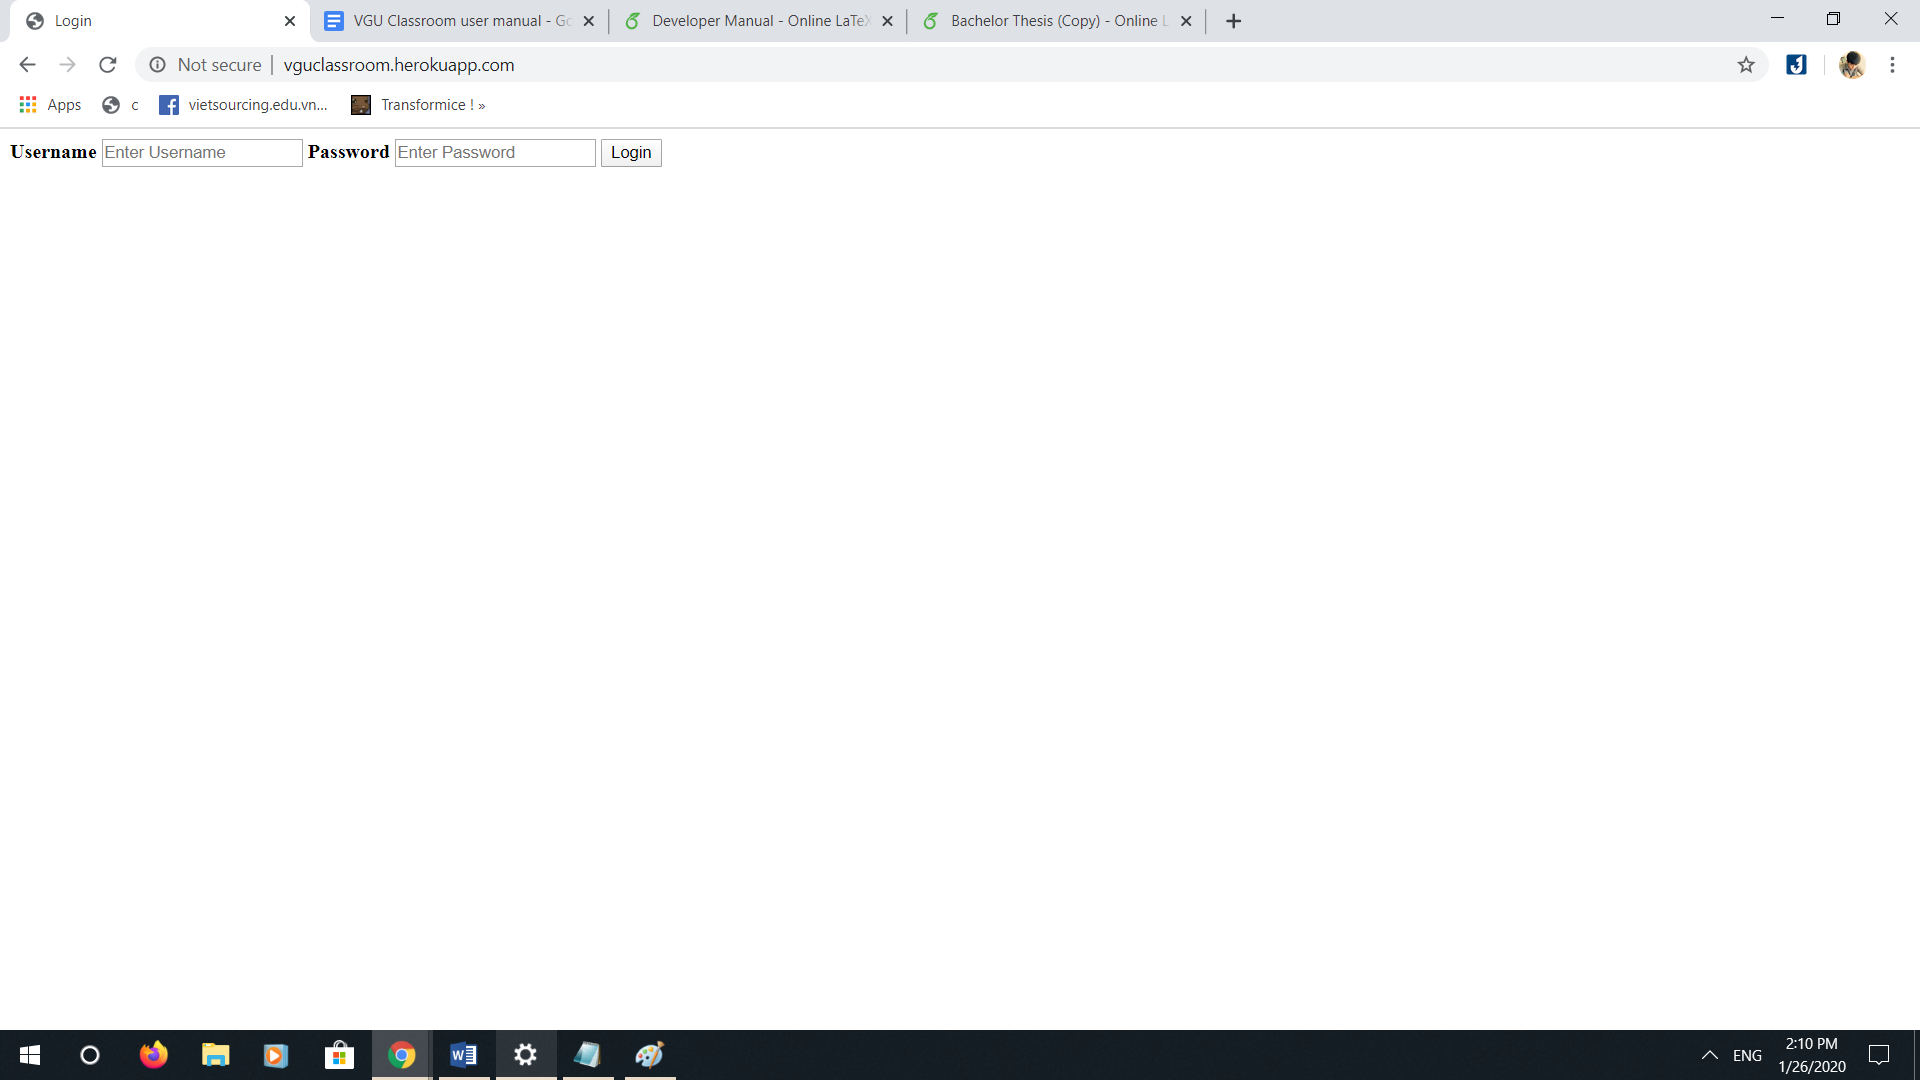
\includegraphics[width=\textwidth,height=\textheight,keepaspectratio]{images/1.png}
\end{figure}
There are just two input fields to input username and password on the login screen. Enter your username and password to log into your account. After you logged in, the app will appear differently based on your account level. There are 3 levels: Administrator, Lecturer and Student.
\section{Administrator}
\begin{figure}[H]
    \centering
    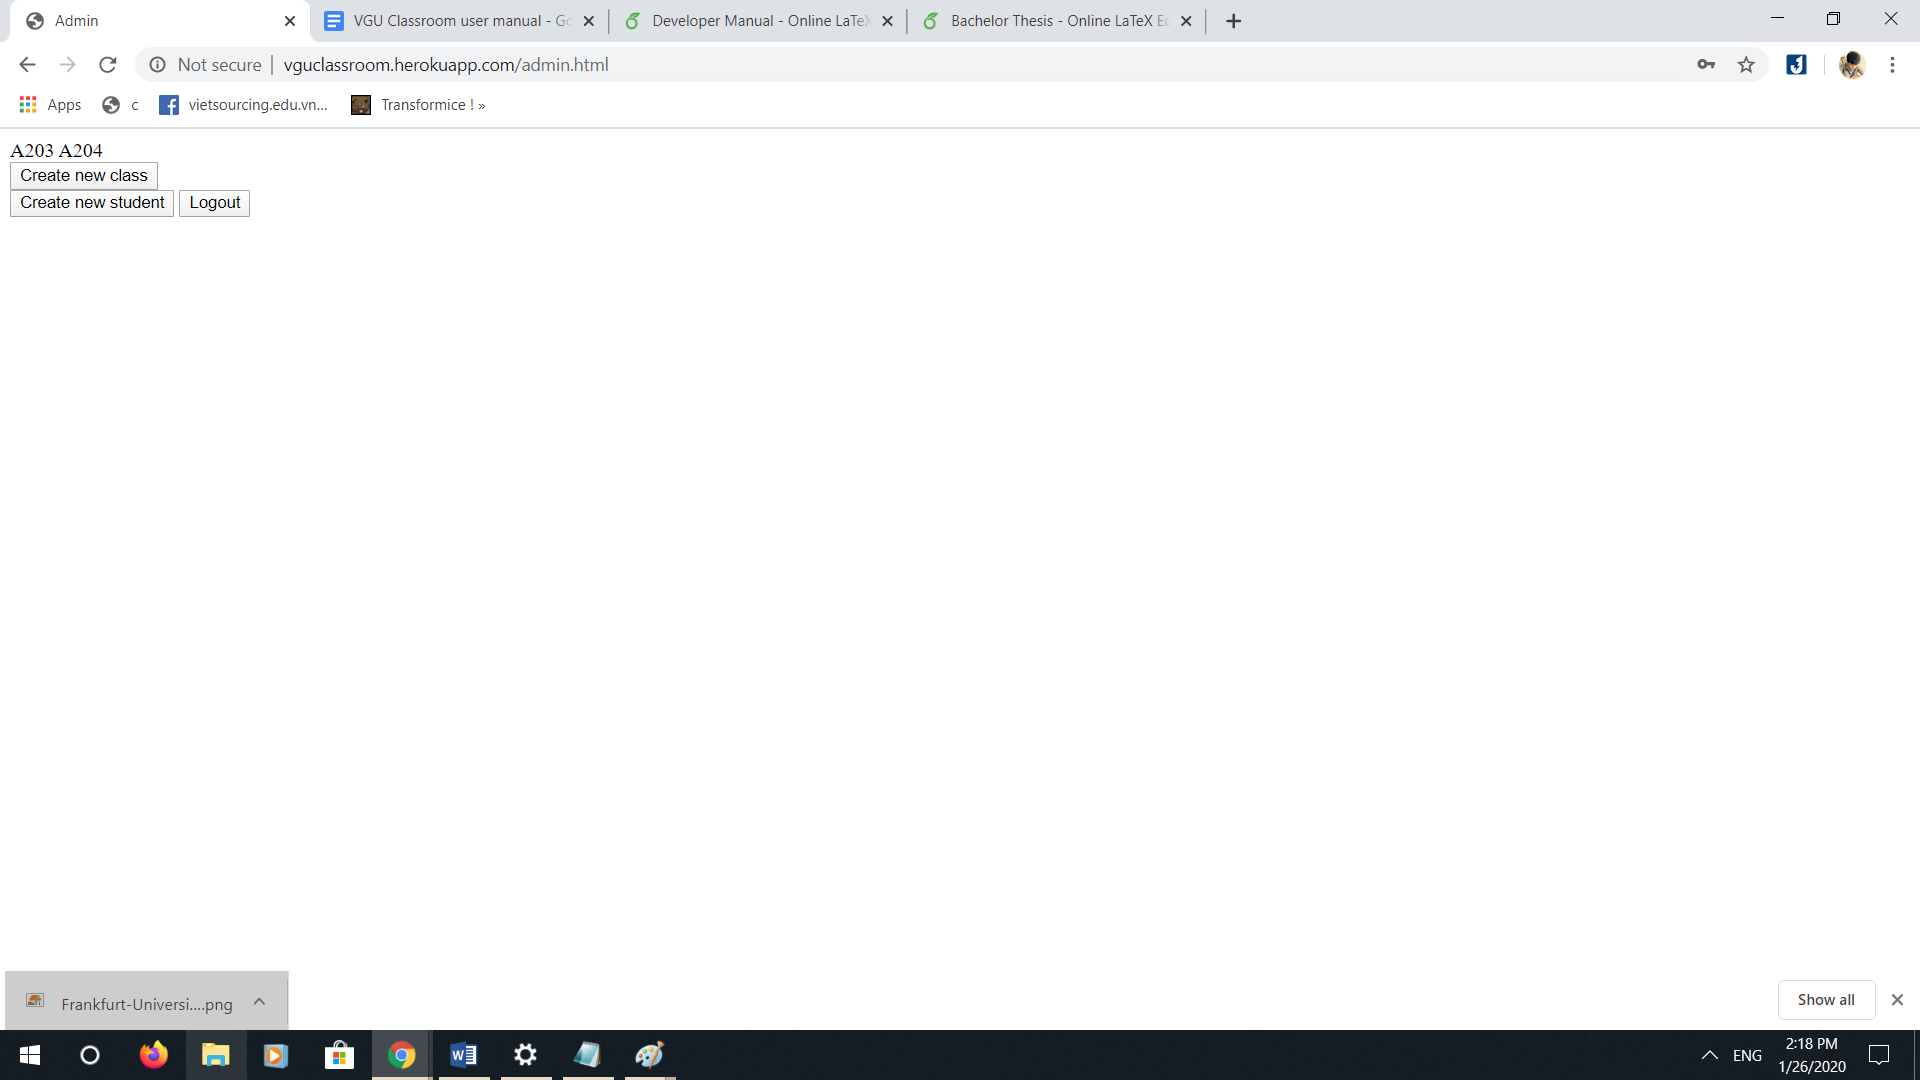
\includegraphics[width=\textwidth,height=\textheight,keepaspectratio]{images/2.png}
\end{figure}
The screen for administrator is simple. The first row states the existing classes. There are  3 buttons, one for creating new class, one for creating new student, and one for logging out.
\subsection{Creating new class}
\begin{figure}[H]
    \centering
    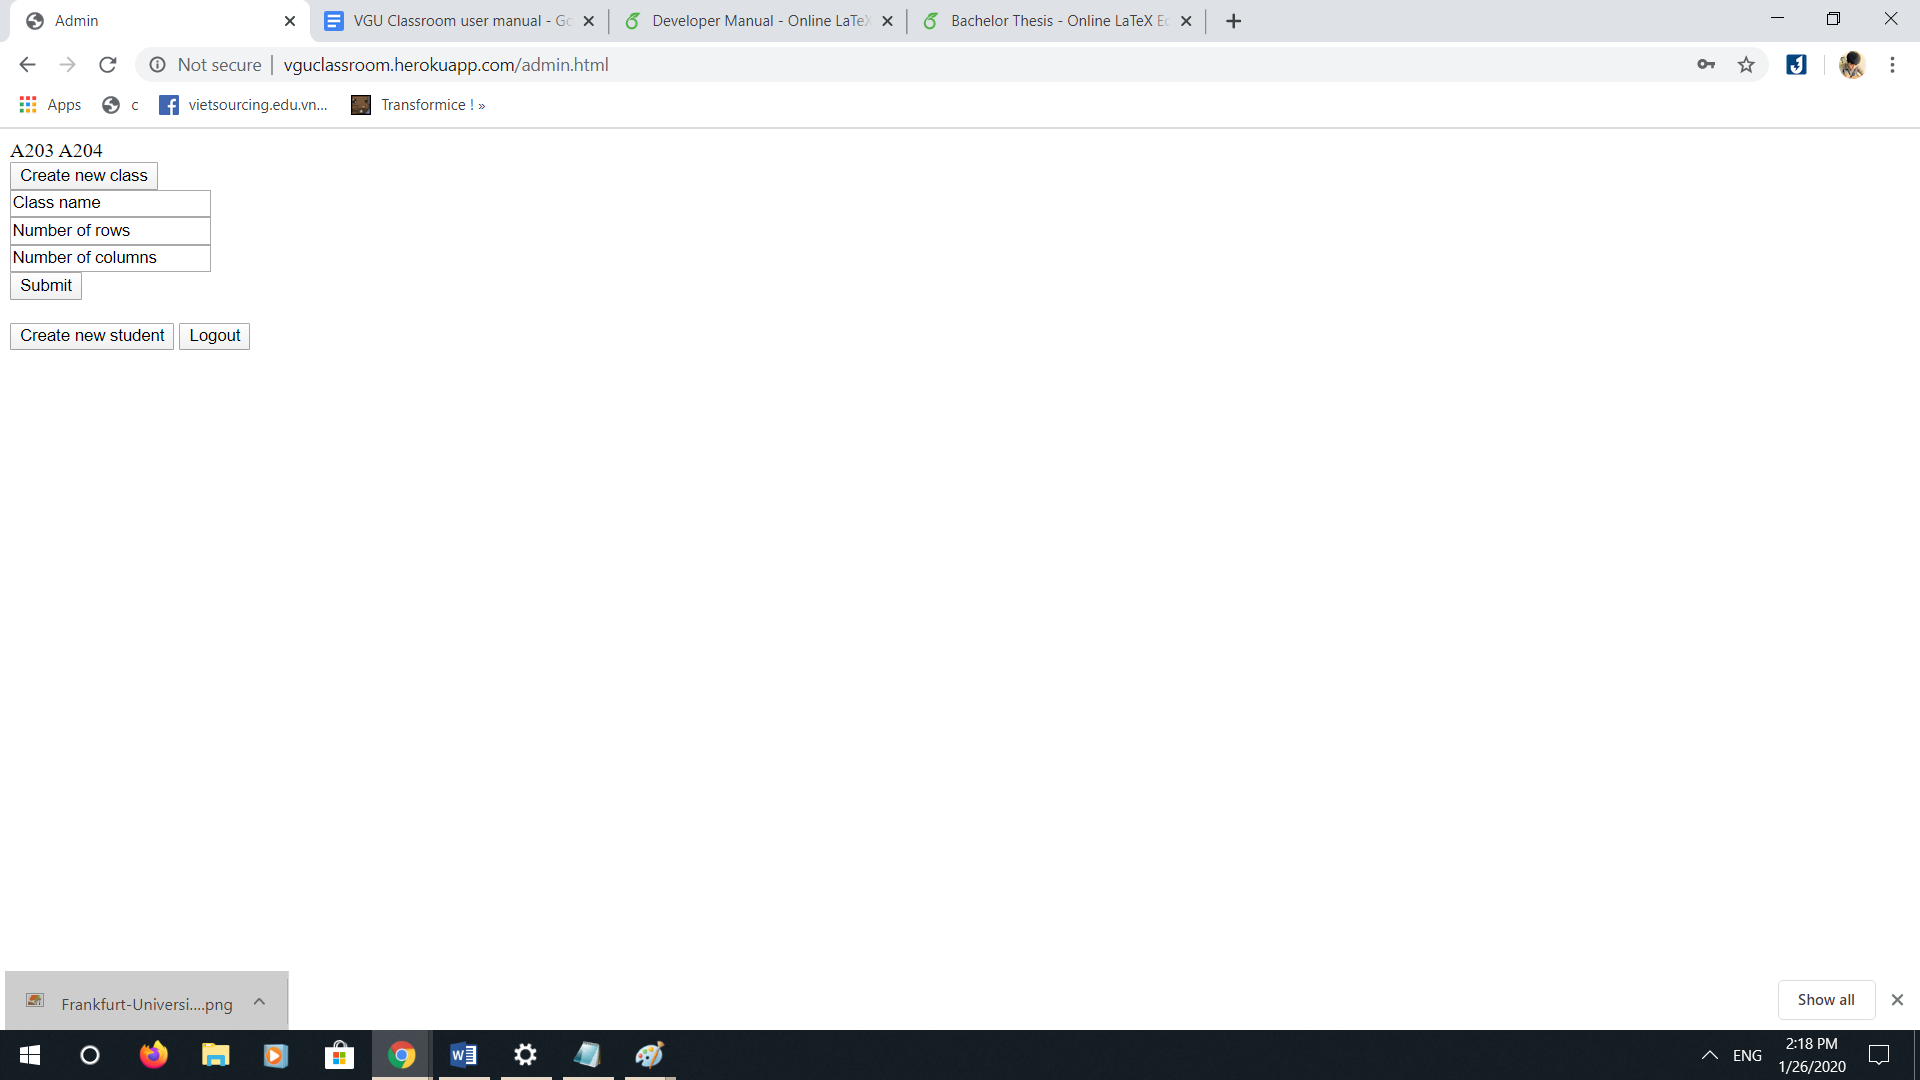
\includegraphics[width=\textwidth,height=\textheight,keepaspectratio]{images/3.png}
\end{figure}
Clicking on the “Create new class” button will show input fields to input the class information. In this application, a seat map of a class is defined as a rectangle. Inputting the right number of rows and columns of seats will help forming the proper “rectangle” of the class map. After inputting all the information needed, click Submit to create a class.
\subsection{Creating new student}
\begin{figure}[H]
    \centering
    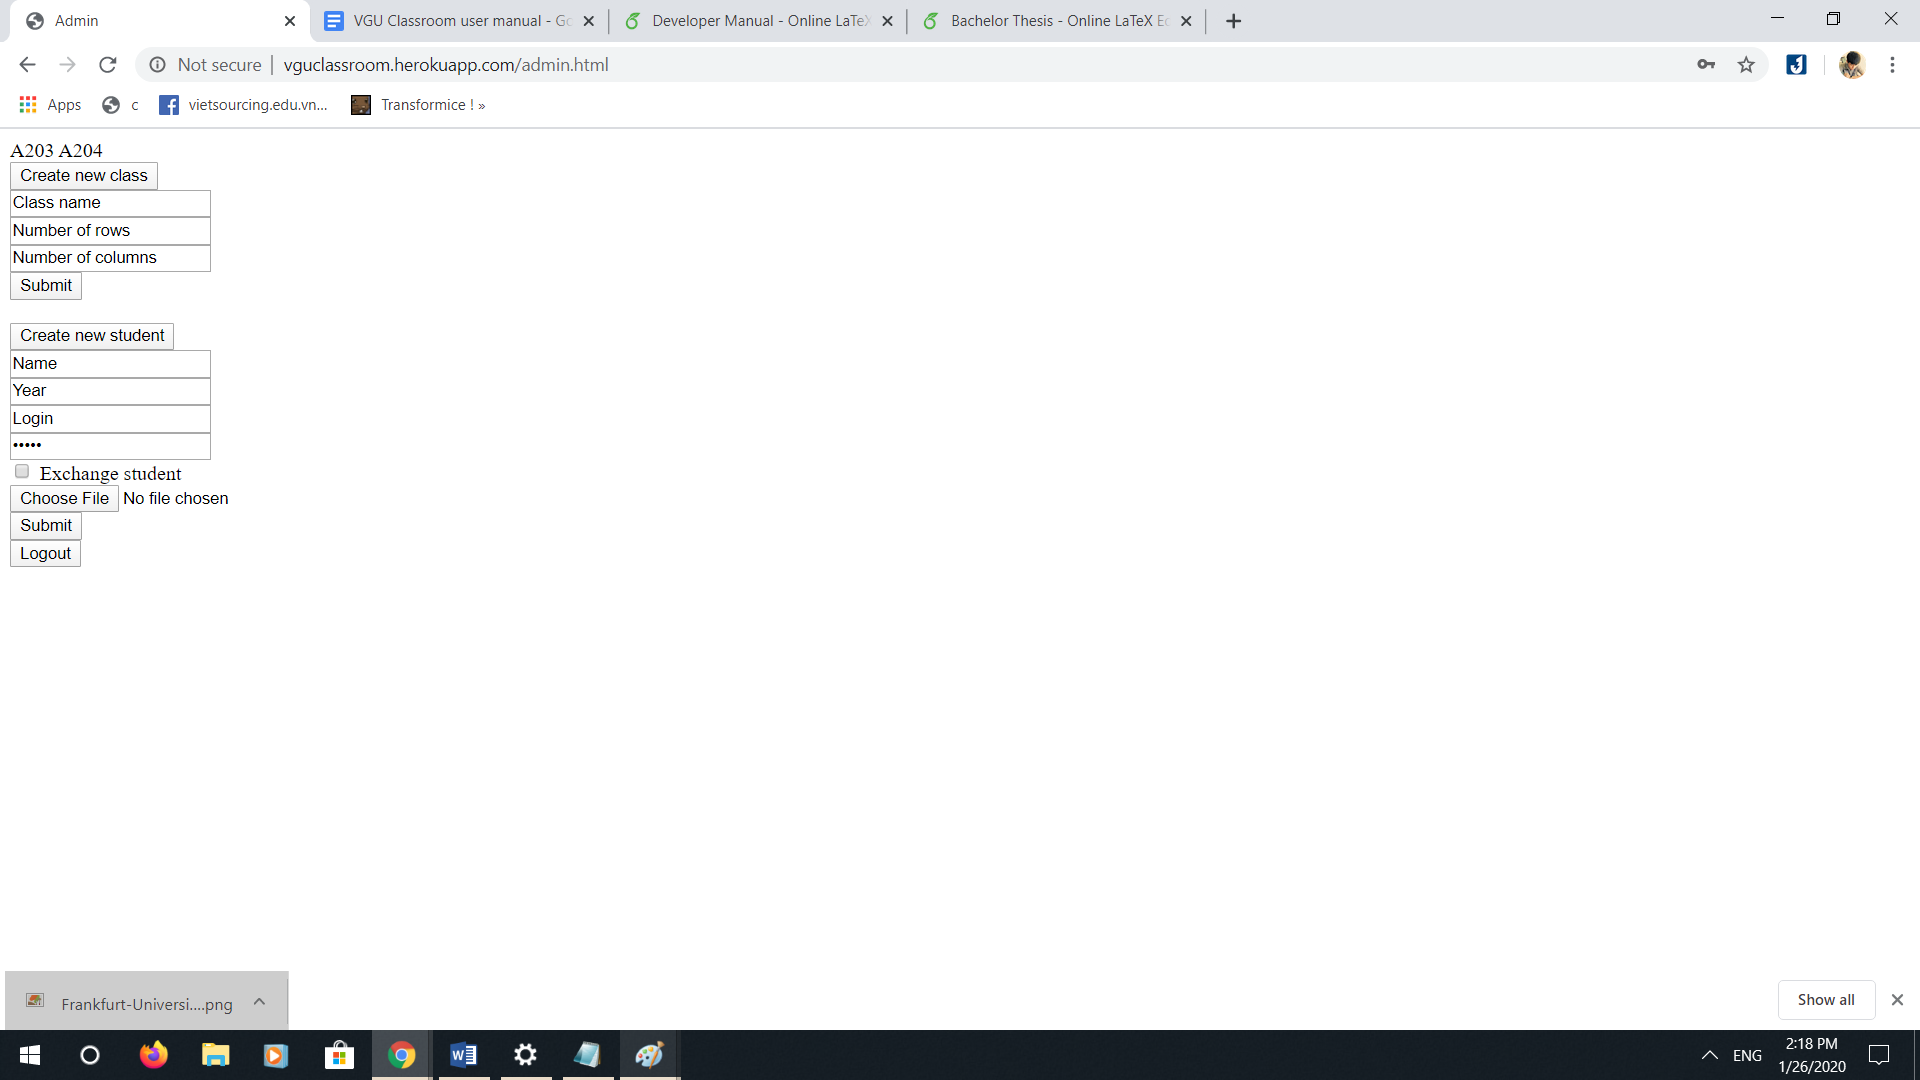
\includegraphics[width=\textwidth,height=\textheight,keepaspectratio]{images/4.png}
\end{figure}
Clicking on the “Create new student” button will show input fields to input the student information. Here, the admin can input the student’s name, intake, username and password for logging into the application, and  a checkbox to check if that student is an exchange student. The admin can also upload the photo of the student. After inputting all the information needed, click Submit to create a student.
\section{Lecturer}
\begin{figure}[H]
    \centering
    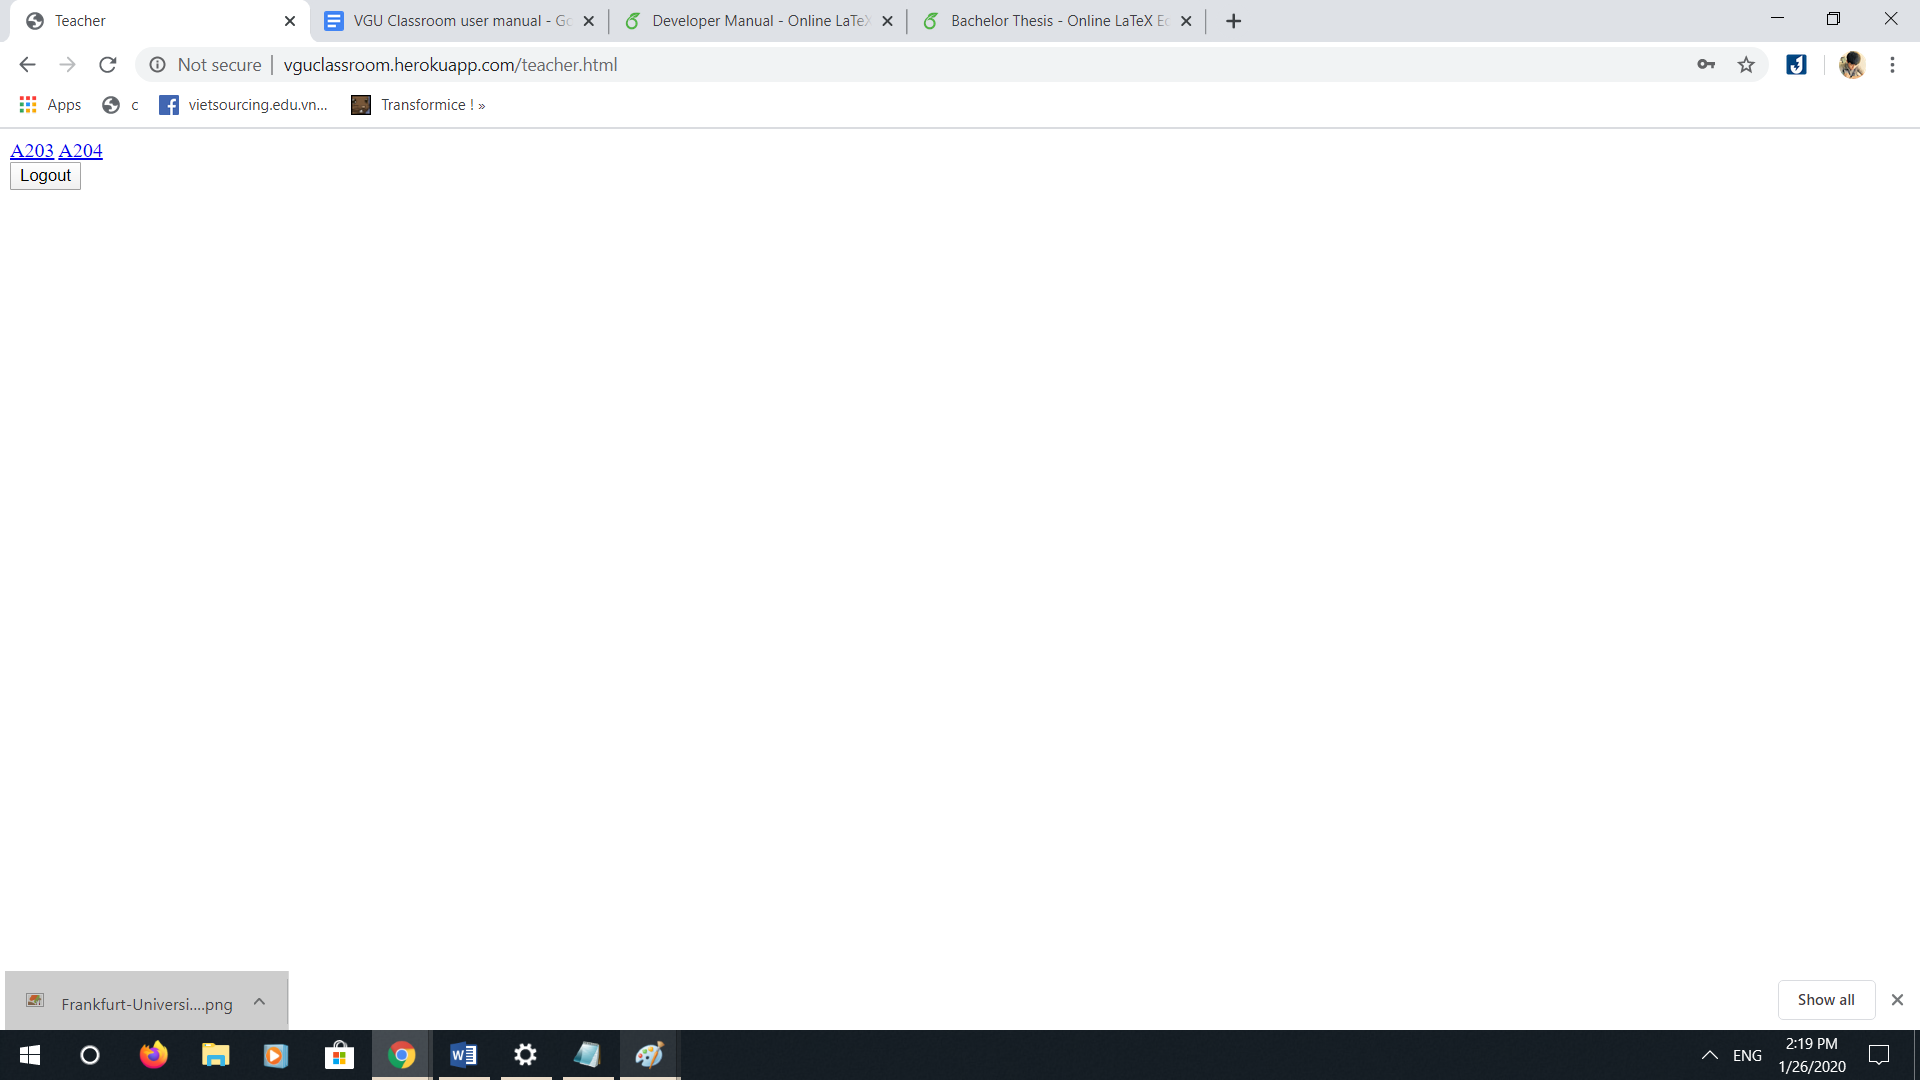
\includegraphics[width=\textwidth,height=\textheight,keepaspectratio]{images/5.png}
\end{figure}
After logging in, the screen of a lecturer is simple, there are just names of the classes that are available. The lecturer can click on a class name to get into that class.
\begin{figure}[H]
    \centering
    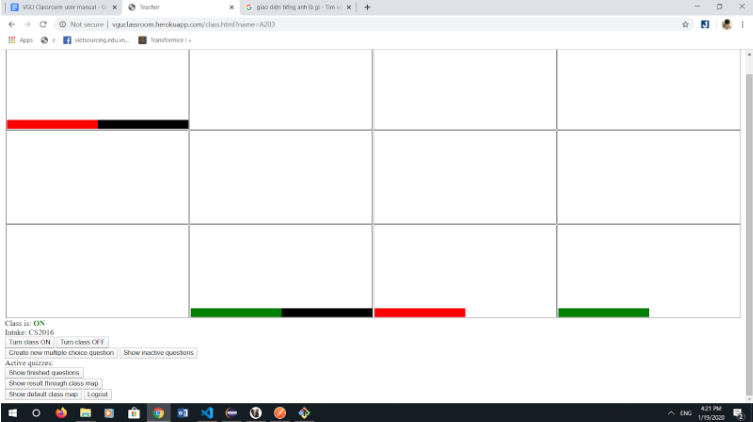
\includegraphics[width=\textwidth,height=\textheight,keepaspectratio]{images/6.png}
\end{figure}
This is the display for a lecturer when he’s in a class. The first thing to see is the class map. The cells that are colored in the bottom represent an occupied seat. If the student is in the same intake with the class, the bottom left frame will be green, otherwise it will be red. If a student is an exchange student, the bottom right frame will be black, otherwise it will be white. If you hover the mouse on an occupied seat, it will show the image and the name of the student sitting in that seat.
\begin{figure}[H]
    \centering
    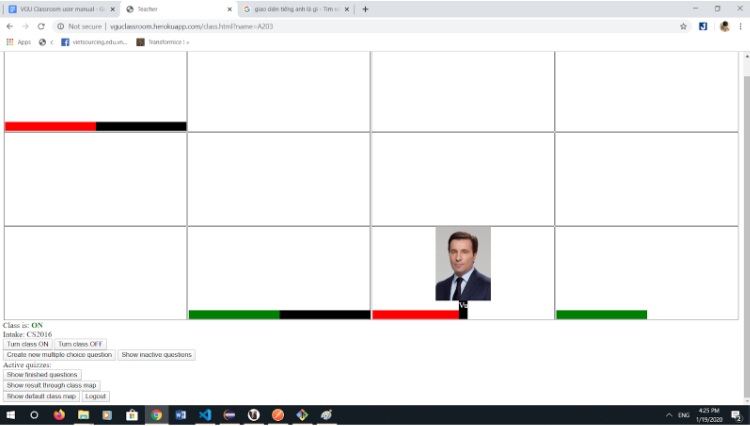
\includegraphics[width=\textwidth,height=\textheight,keepaspectratio]{images/7.png}
\end{figure}
Let’s take a look at the information of the students who are taking the class:
\begin{figure}[H]
    \centering
    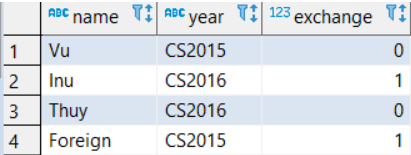
\includegraphics[width=\textwidth,height=\textheight,keepaspectratio]{images/8.png}
\end{figure}
First, we will consider the frame for Vu:
\begin{figure}[H]
    \centering
    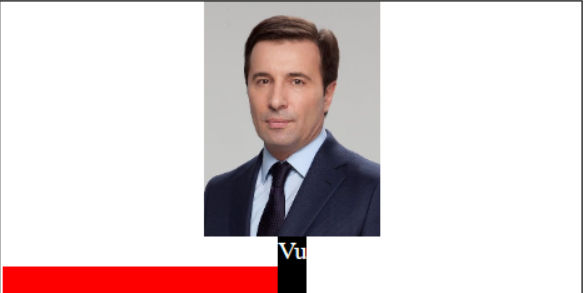
\includegraphics[width=\textwidth,height=\textheight,keepaspectratio]{images/9.png}
\end{figure}
As we can see from the information table, Vu’s intake is CS2015, and he is not an exchange student. The above capture of the screen shows that, the intake that is taking the class is CS2016, therefore Vu is not in the same intake with the class, which colored the bottom left frame red. Since Vu is not an exchange student, the bottom right frame is white.\par 
For the frame of Inu:
\begin{figure}[H]
    \centering
    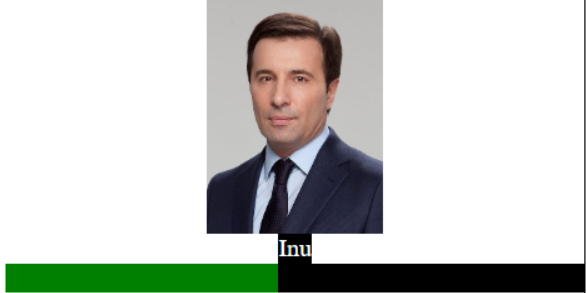
\includegraphics[width=\textwidth,height=\textheight,keepaspectratio]{images/10.png}
\end{figure}
Inu’s intake is CS2016, and he is an exchange student. He is in the same intake with the class, so the  bottom left frame is green, and he is an exchange student, so the bottom right frame is black.\par 
For the frame of Thuy:
\begin{figure}[H]
    \centering
    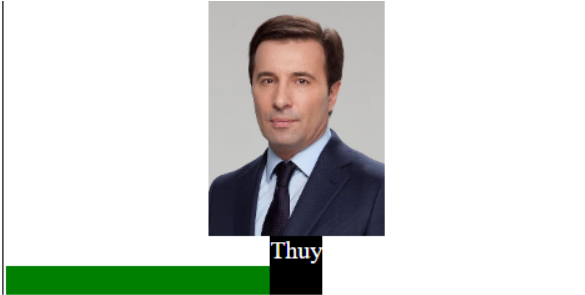
\includegraphics[width=\textwidth,height=\textheight,keepaspectratio]{images/11.png}
\end{figure}
Thuy’s intake is CS2016, the same intake with the class, and he is not an exchange student. Therefore, the bottom left frame is green, and the bottom right frame is white.\par 
For the frame of Foreign:
\begin{figure}[H]
    \centering
    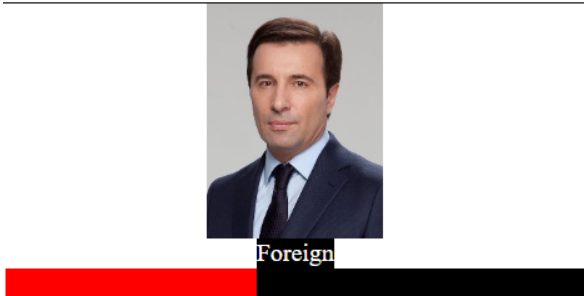
\includegraphics[width=\textwidth,height=\textheight,keepaspectratio]{images/12.png}
\end{figure}
Foreign’s intake is CS2015, not the same intake with the class, and he is an exchange student, so the bottom left frame is red, and the bottom right frame is black.\par 
Below the class map, there are texts showing the state of the class, the intake taking the class, and buttons that the lecturer can click on to use his functions:
\begin{figure}[H]
    \centering
    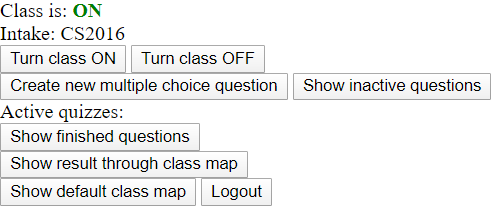
\includegraphics[width=\textwidth,height=\textheight,keepaspectratio]{images/13.png}
\end{figure}
\subsection{Turning a class on and off}
A class always has its default state as OFF. If the teacher wants the student to join the class, he will have to turn the class on first. Clicking the “Turn class ON” button will show a text field to input the Intake that is taking the class. After inputting this, click “Submit the intake and turn class ON” to turn on the class. After the lecture, the lecturer can turn the class off by clicking the “Turn class OFF” button. All seats taken by the student will be available again after turning the class off.
\begin{figure}[H]
    \centering
    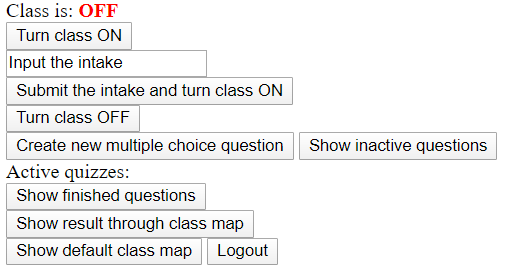
\includegraphics[width=\textwidth,height=\textheight,keepaspectratio]{images/14.png}
\end{figure}
\subsection{Quiz}
In this application, a quiz only has one multiple choice question. You can create a new quiz by clicking the “Create new multiple choice question” button.
\begin{figure}[H]
    \centering
    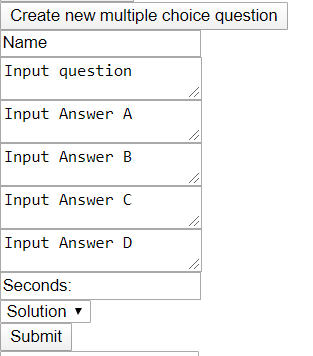
\includegraphics[width=\textwidth,height=\textheight,keepaspectratio]{images/15.png}
\end{figure}
After clicking the button, the application will show fields that the lecturer needs to fill in to create the quiz. The required fields are the name of the quiz, the question of the quiz, the four choices, the time allotted for the quiz, and the right solution. After filling those fields, the lecturer can click Submit to create the quiz. A newly created quiz is an \textbf{inactive} quiz. The lecturer can click on the “Show inactive questions” button to see all inactive quizzes.
\begin{figure}[H]
    \centering
    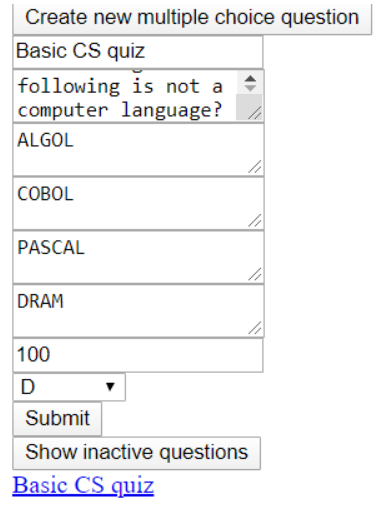
\includegraphics[width=\textwidth,height=\textheight,keepaspectratio]{images/16.png}
\end{figure}
Click on the link to come to the page displaying that quiz.
\begin{figure}[H]
    \centering
    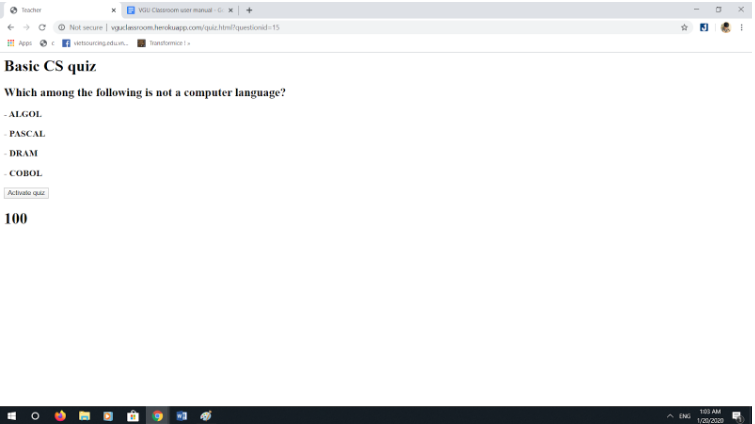
\includegraphics[width=\textwidth,height=\textheight,keepaspectratio]{images/17.png}
\end{figure}
The page displaying a quiz will consist of its name, its question, its answers (the orders are randomized, so it will not be the same with the order when the lecturer first input the quiz), a button to activate the quiz, and a timer for a quiz. The lecturer can click the button to activate the quiz, so the students can start doing it. The timer will begin to work when the quiz is activated. After the timer runs out, the quiz is \textbf{finished}.\par 
When a quiz is \textbf{active}, the teacher can see a live update of students doing the quiz by clicking the button holding the name of the quiz.
\begin{figure}[H]
    \centering
    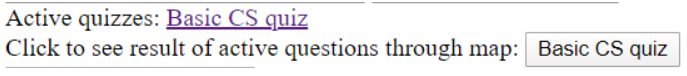
\includegraphics[width=\textwidth,height=\textheight,keepaspectratio]{images/18.png}
\end{figure}
Apart from being capable of live updating, the result of this button is the same with the function for the “Show result through class map” button, so it will be discussed later.\par 
Let’s have an example. The four abovementioned students did the quiz, and this is the result. (N is for “no answer”). From this table, Vu and Thuy did the quiz right, Inu got it wrong, and Foreign had no answer.
\begin{figure}[H]
    \centering
    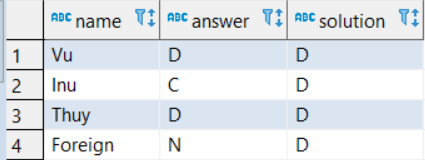
\includegraphics[width=\textwidth,height=\textheight,keepaspectratio]{images/19.png}
\end{figure}
The teacher can click on the “Show finished questions” to show the finished quizzes. Links of the finished quizzes will appear.
\begin{figure}[H]
    \centering
    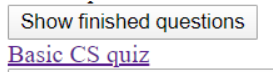
\includegraphics[width=\textwidth,height=\textheight,keepaspectratio]{images/20.png}
\end{figure}
Click on the link to see the average result of the quiz.
\begin{figure}[H]
    \centering
    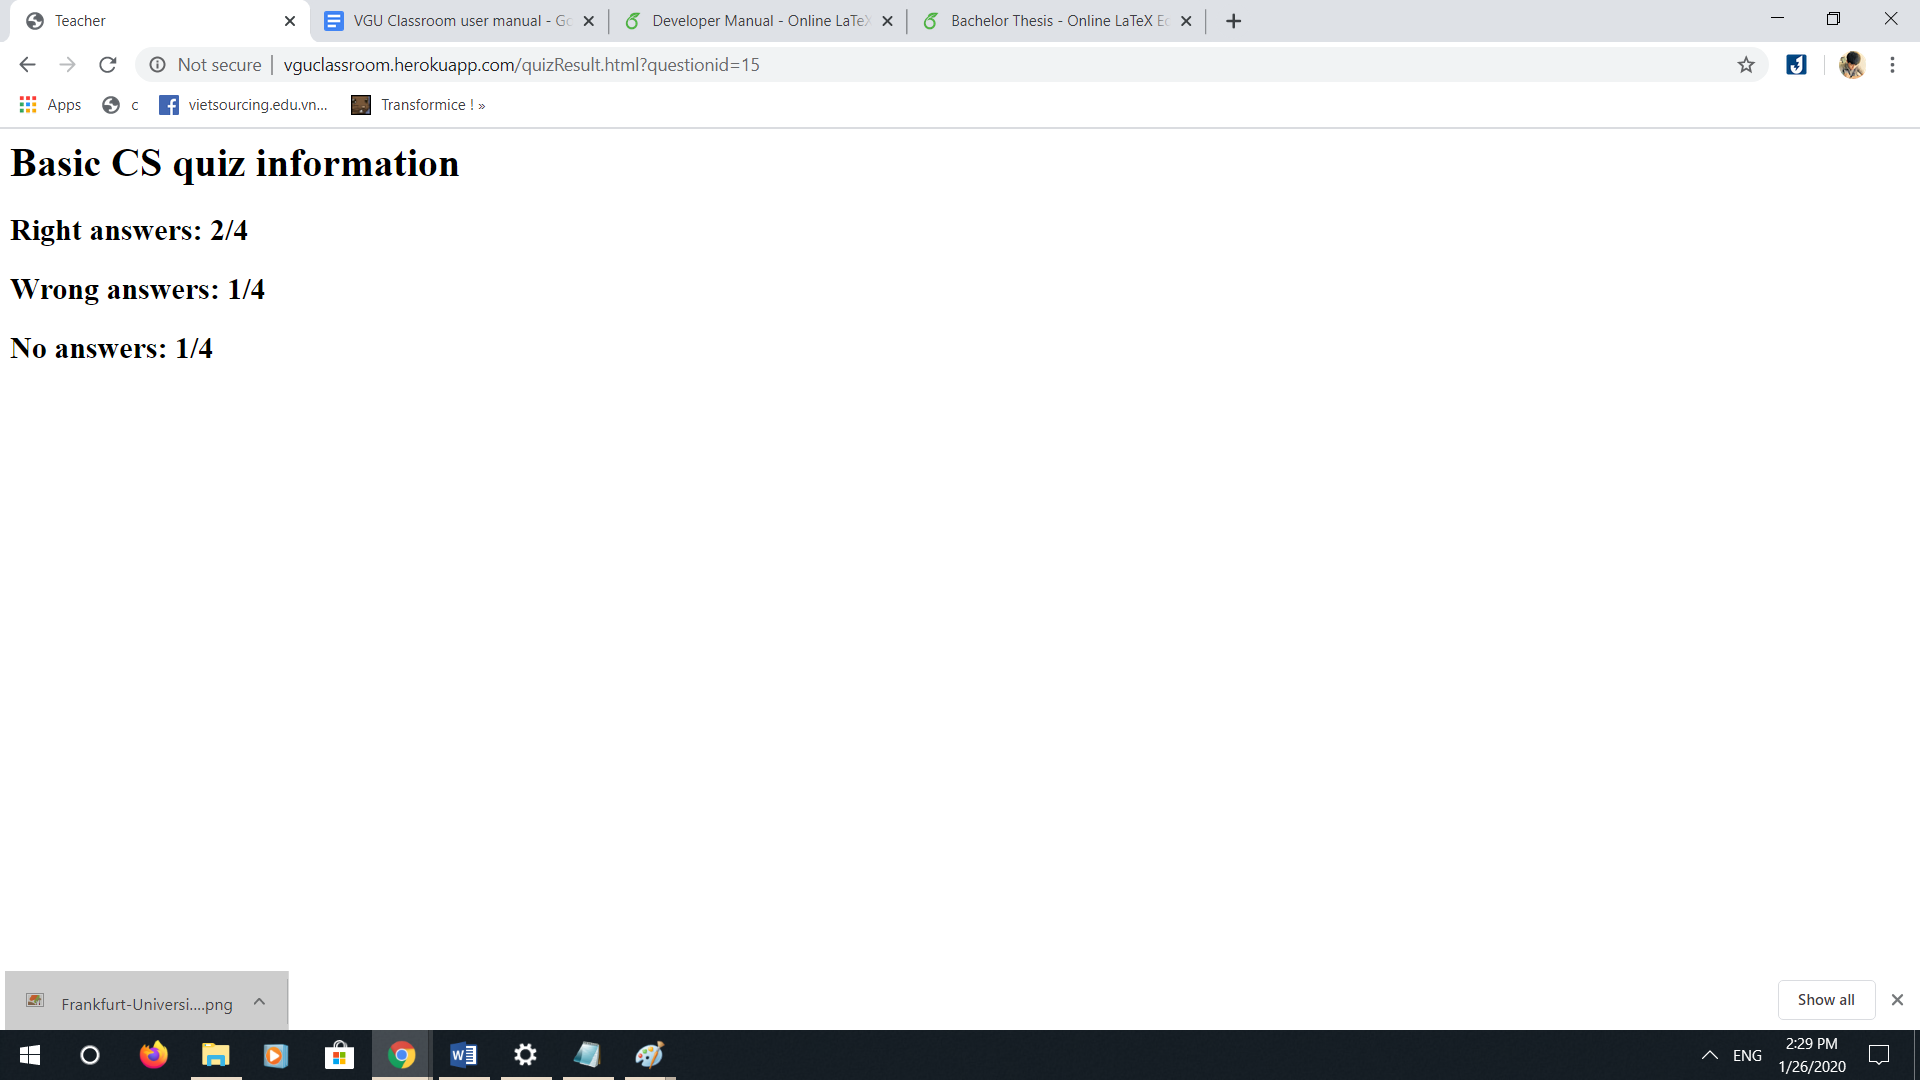
\includegraphics[width=\textwidth,height=\textheight,keepaspectratio]{images/21.png}
\end{figure}
There are 4 students in the class at that moment, so the total number of students taking the quiz is 4. Vu and Thuy got it right, so there are 2 right answers out of 4. Inu was wrong, so there is 1 wrong answer. Foreign could not answer it in time, so there is 1 student who had no answer.\par 
Besides this page which shows the average result of the quiz, the teacher can also see the result of the quiz through the class map by clicking “Show result through class map”. It will show buttons representing the finished quizzes.
Click on the button representing a finished quiz to see the result of that quiz through class map.
\begin{figure}[H]
    \centering
    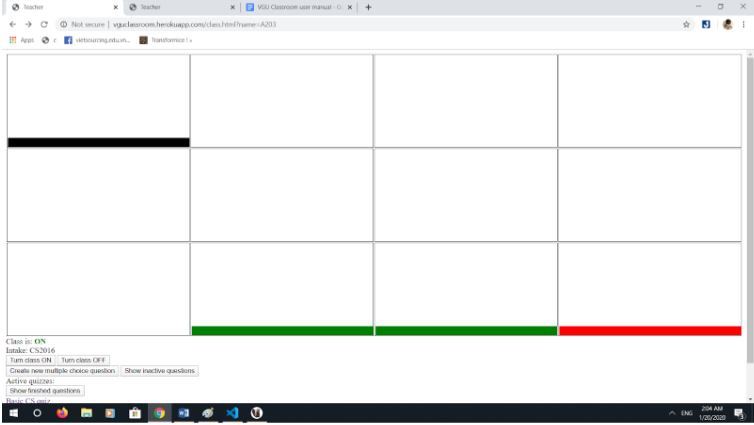
\includegraphics[width=\textwidth,height=\textheight,keepaspectratio]{images/22.png}
\end{figure}
Vu and Thuy got the right answer, so their seat is colored green. Inu got the wrong answer, so their seat is colored red. Foreign did not have the answer, so his seat is black. The lecturer can also revert back to the normal class map by clicking “Show default class map.”
\section{Student}
Upon logging in, the student will see the available classes, and the quizzes done by them. A student can click on a quiz to review that quiz, or click on a class to get into that class.
\subsection{Quiz review}
\begin{figure}[H]
    \centering
    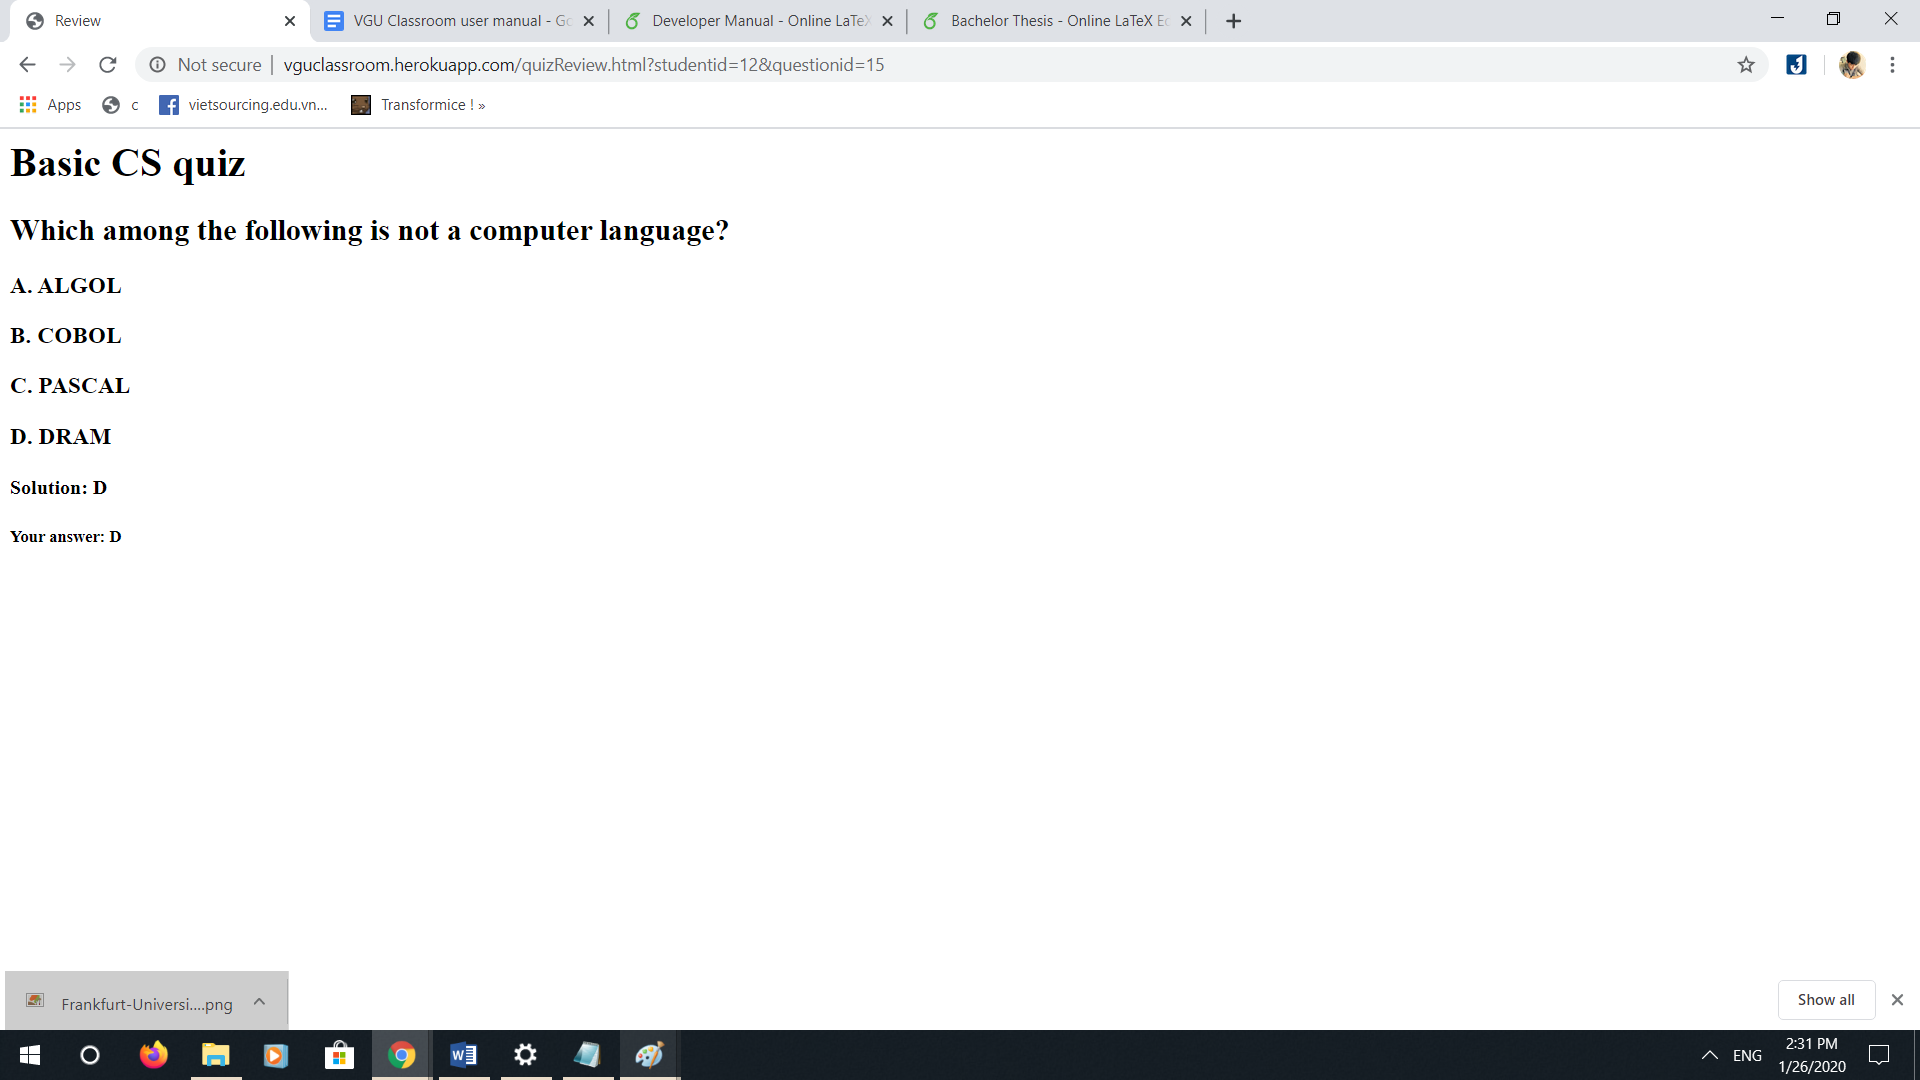
\includegraphics[width=\textwidth,height=\textheight,keepaspectratio]{images/23.png}
\end{figure}
The quiz review screen shows the name of the quiz, the question, all the choices, the right solution, and the student’s answer
\subsection{Class}
\begin{figure}[H]
    \centering
    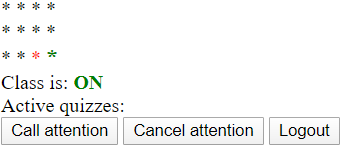
\includegraphics[width=\textwidth,height=\textheight,keepaspectratio]{images/24.png}
\end{figure}
This is the display of a class for a student in the application. Since students do not need to see as much information of other students like the lecturers, the class map here is just represented by stars. Black stars are for the unoccupied seats, red stars are for occupied seat, and the larger green star is for the seat that the user is sitting in. To occupy a seat, a user can click on the black star representing that seat. Occupied seat cannot be occupied by another student. If a student, who already occupied a seat, occupies another seat, his old seat will be left free, and will become a black star again. \par 
If there is an active quiz during class, the application will update it immediately to the student by a link next to the text “Active quizzes”. The student can click on the link to go to the quiz.
\begin{figure}[H]
    \centering
    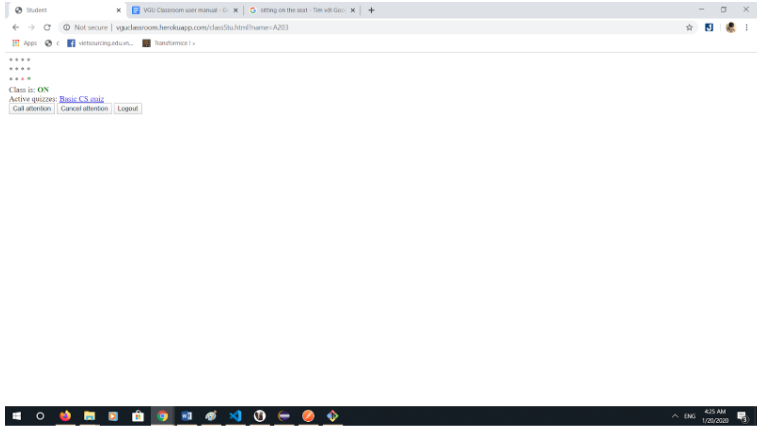
\includegraphics[width=\textwidth,height=\textheight,keepaspectratio]{images/25.png}
\end{figure}
The page for the test will show the name of the test, the question, and the choices appearing in a random order. To complete the quiz, the student can check on the right answer, and click “Submit answer” before the timer runs out
\begin{figure}[H]
    \centering
    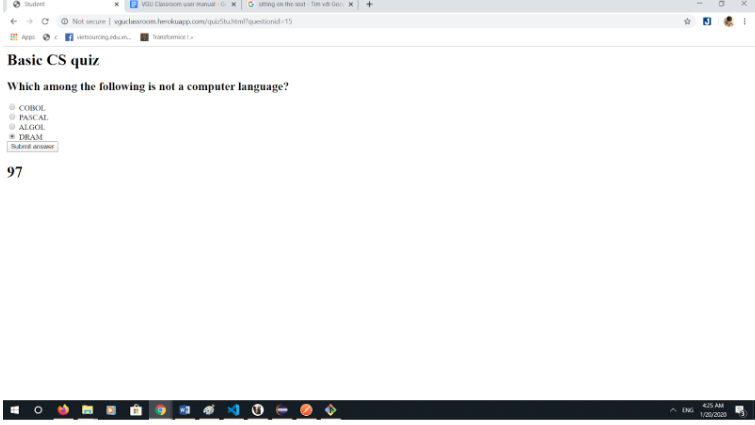
\includegraphics[width=\textwidth,height=\textheight,keepaspectratio]{images/26.png}
\end{figure}
In the page of the Class, the student can click on the button “Call attention” to call for the attention of the lecturer, without having to wave their hand, or call for the lecturer by their voice. When a student is calling for attention, their seat on the lecturer’s display will turn red, and the lecturer will hear beeping sound to alarm them that there is a student calling for them.
\begin{figure}[H]
    \centering
    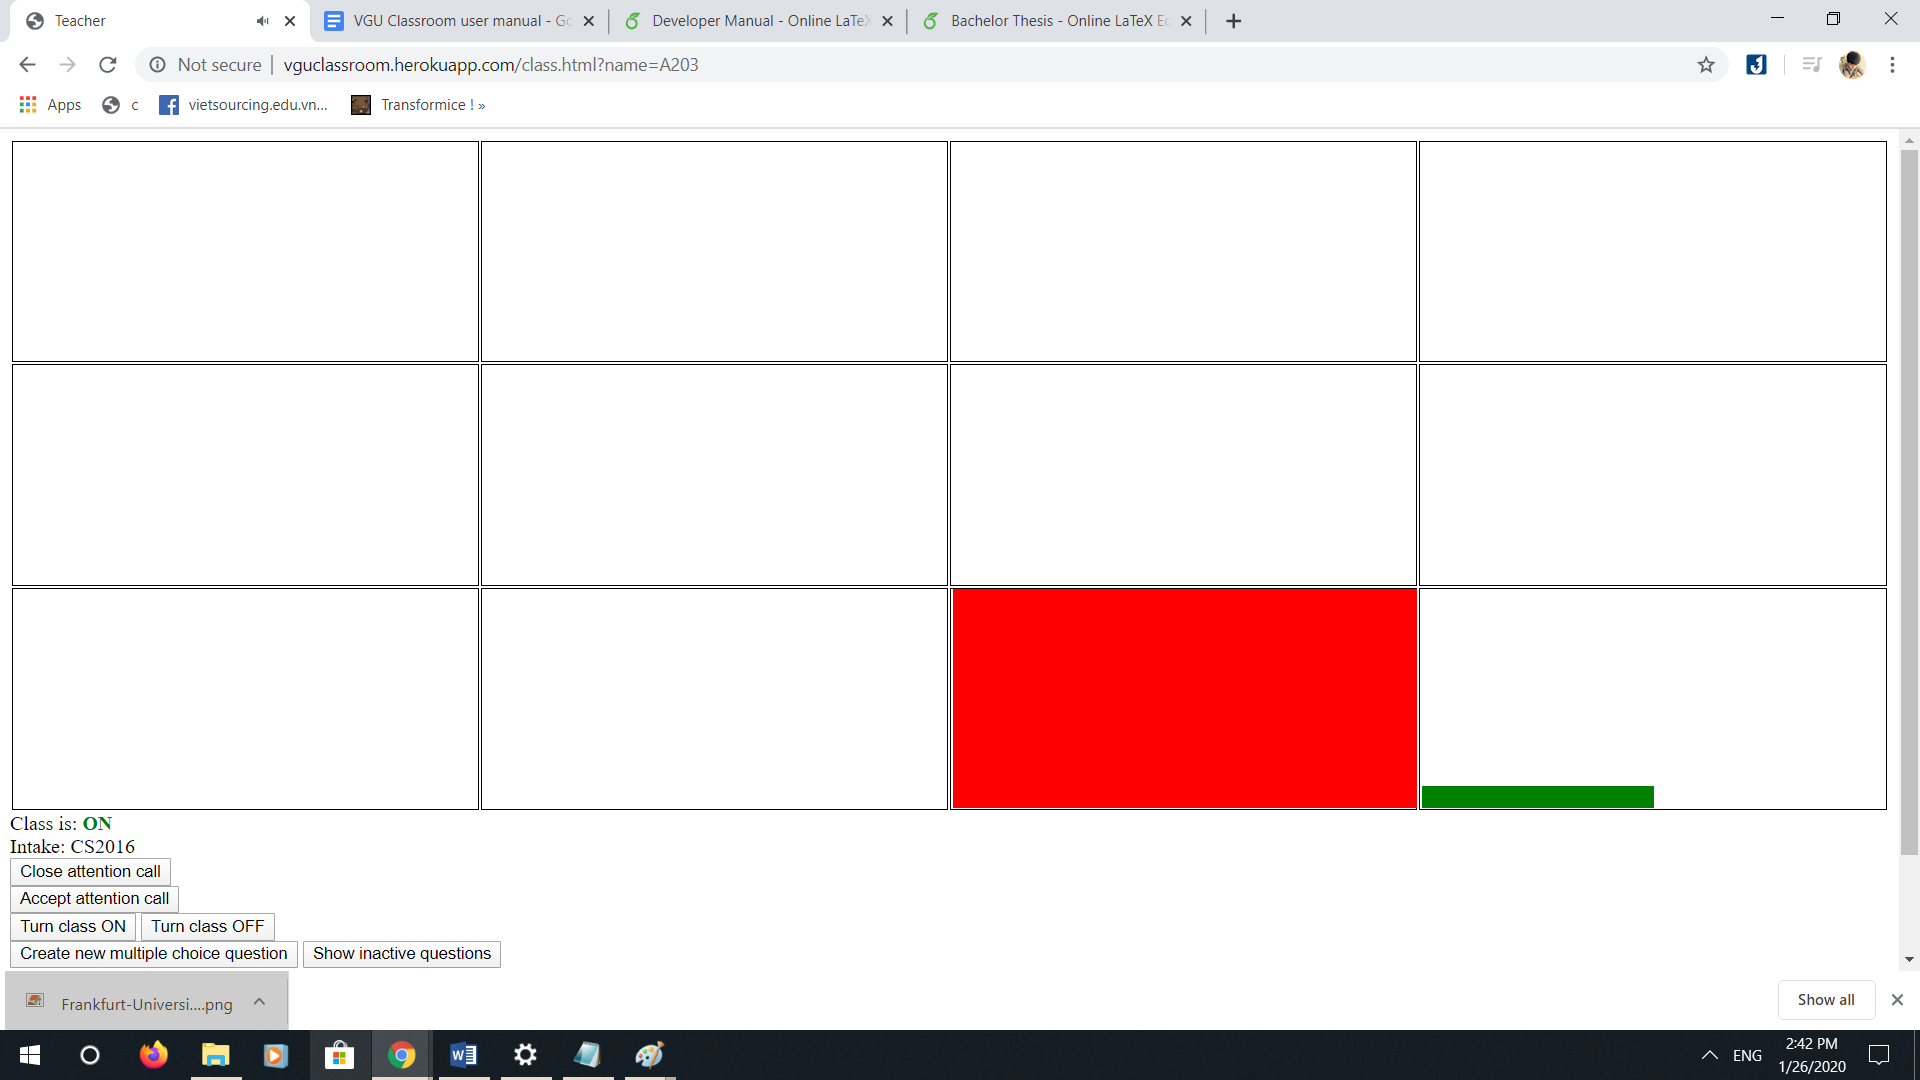
\includegraphics[width=\textwidth,height=\textheight,keepaspectratio]{images/27.png}
\end{figure}
The student can also close the attention call with the button “Cancel attention”	

\chapter{Developer manual}
\section{Web app}
A web app is an application that applies the client-server model, where the client is the browser and the server is the webserver. The Hypertext Transfer Protocol (HTTP) is applied for transaction of data over systems of connections. With this concept, the users do not have to count on any particular Operating System (OS) or hardware configuration. Therefore, web apps are able to support services that are cross-platform.\par
In a web app, all data and logic exist in the basis domain server. The app can be connected to with any browser, and without installation. Redistributing, administrating and preserving the app on multiple OS, which are the time-consuming processes of the development of a desktop app, are not necessary in web apps. The process to develop a web app bears 2 parts: Client-side and Server-side, which are often called Front-end and Back-end, respectively.

\subsection{Front-end}
A front-end developer is the one who is in charge of developing the graphical user interface arrangement of a site. The process of front-end developing is crucial on account of the fact that the user interface is the sole place that the users can communicate with the app. In this process, I used
HyperText Markup Language (HTML), Cascading Style Sheets (CSS), and JavaScript (JS).\par

\begin{itemize}
    \item HTML: The approved markup language for webpages, whose elements  are the components of HTML pages.\cite{html}
    \item CSS: This defines how HTML elements are to be presented. \cite{css}
    \item JavaScript: The programming language for the Web. HTML and CSS can be interacted with by JavaScript. It can be used to compute, handle and authenticate data. \cite{js}
\end{itemize}

\subsection{Back-end}
Back-end development generally aims attention at the logic and services of the web app. As the gist of the web app, it basically stores and executes all the functionalities of the application. It operates the data from the front-end, and sends back the outcome to the front end in a comprehensible manner. \par

A web server develops the back-end of the app. The mission of the web server is that, it delivers data for the clients, which, for the most part, are the browsers. There are various elements that make up a web server, and the center of it is an HTTP server. This HTTP server is a computer program that realizes the concept of URL and the protocol of HTTP. One can understand the fundamental concept of this process by looking at the following figure:

\begin{figure}[H]
    \centering
    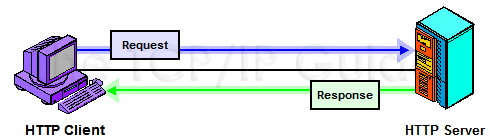
\includegraphics{images/httpclientserver.png}
    \caption{HTTP Client/Server information exchanging}
    \label{fig:protocalExample}
\end{figure}
From the figure, we can see the steps of the process as follows:
\begin{enumerate}
    \item A connection with the Server is created by the Client using the protocol of HTTP.
    \item Client transmits a request for data from Server.
    \item A response is returned to the Client, transferring back the data.
\end{enumerate}
This process comes with a fixed array of principles:
\begin{itemize}
    \item The server shall respond to the client's request exclusively, and it cannot deliver requests to the client. 
    \item It is necessary for the server to respond to all arriving requests. Alternatively, a timeout message will be sent to the client, signifying that the server has not replied within the particularized time.
    \item Each request needs to include a URL address that displays a specific service 
\end{itemize}
\subsection{Multiple-Page Application}
Since the functions of the application can be accessed differently by three roles, and there are functions that should be viewed in different pages, putting the pattern of Multiple-Page Application into use is convenient for the application development. Multiple-Page Applications are the classic web apps that refresh the whole page and show a new one upon getting communicated with by the users. This pattern is good with the search engine, and it supplies an observable outline of the application to the user.\cite{mpa}
\subsection{Web workers}
A web worker is a JavaScript that operates behind-the-scenes. It runs separately from other scripts without influencing the efficiency of the page. Rendering a new web worker additionally creates new threads to carry out that JavaScript code. As a result, a multi-thread architecture is efficiently developed, in which an application may accomplish multitasking. \par
In my application, 4 web workers are used for the following functions:
\begin{itemize}
    \item 1 worker for the live update of students doing the quiz through class map for the lecturer.
    \item 2 workers for the function of Attention Call. (one worker is to update for the teacher that if there is any student calling him, and another is to update for the student that if their call is accepted by the teacher)
    \item 1 worker for the live update of active quizzes for the students.
\end{itemize}
\subsection{JSON Web Token}
JSON Web Token (JWT) is an open standard that gives description to a solid and independent method for a secured communication between partakers as a JSON Object. The information transmitted in the communication can be confirmed and trusted because it is digitally signed. In my application, the JWTs are signed applying a secret (with the HMAC algorithm). \par

JWTs are made up of three components split by dots (.), which are the Header, the Payload, and the Signature. For that reason, a JWT usually appears like this: xxxxx.yyyyy.zzzzz\par

The header commonly contains two parts: the type of the token, which is JWT, and the signing algorithm. In my application, I used HMAC SHA256.
\begin{tabbing}
\verb|{| \\
\quad \verb|"alg"| : "HS256", \\
\quad  \verb|"typ"| : "JWT" \\
\verb|}|
\end{tabbing}
This JSON is Base64URL encoded to make the first part of the JWT\par
The payload makes the second part of the JWT, which holds the declarations about the user.
In my application, a payload will look like this:
\begin{tabbing}
\verb|{| \\
\quad \verb|"id"| : 1, \\
\quad  \verb|"role"| : 1 \\
\verb|}|
\end{tabbing}
Like the header, this JSON is also Base64URL encoded to make the second part of the JWT.\par
To construct the signature, you must sign the encoded header and payload with a secret and the algorithm designated in the header. The signing function will be: Algorithm(base64UrlEncode(header) + "." + base64UrlEncode(payload), secret). This signature is to validate: (1) the message was not adjusted while being sent, and (2) the sender of the JWT.
In my application, when the user inputs the right username and password to login, they will earn a JSON Web Token. At whatever time the user desires to use a function, the user agent should send the JWT in the Authorization header employing the Bearer schema. The header should resemble this:\par
Authorization: Bearer (token)\par
The server will inspect for a genuine JWT in the Authorization header, and if it exists, the user will be permitted use the functions based on their role, which is stated in the payload of the JWT.\cite{jwt}

\section{Library and Framework}
\subsection{Overview}
JavaScript and Java, two of the most well-known programming languages, are used during the whole of the application development, with JavaScript being used to make the front-end, and Java is used for the back-end. JavaScript is an all-powerful language that can do many things for a website, like powering the site's common interactivity. It allows the site to have extra services that is not alternatively doable with just HTML and CSS. It favors the webpages to "answer" the actions of the users and vigorously update themselves. Although my application is a multipage web app, there also are functions that can work on one page, and JavaScript makes it possible for a function to complete without asking for a page refresh.\cite{js2} \par
For the back-end, I used Spring Boot. Before discussing Spring Boot, first, we have to look at the definition of the Spring Framework. It is a Java platform that brings thorough infrastructure backing for developing Java apps. It manages the infrastructure so the developer can concentrate on the app itself.\cite{spring} \par
Spring Boot is a Java-based framework used to develop a stand-alone and production-grade Spring application that you can run with least configurations, compared to the complicated configuration setup of the Spring framework.
Spring Boot has many advantages, and the followings are the ones that made me pick Spring Boot as my first choice in the process of developing the back-end of the application:
\begin{itemize}
    \item It stays away from the complicated XML configuration of the Spring Framework.
    \item It is effective in controlling REST endpoints.
    \item It presents annotation-based Spring application.
    \item It helps dependency control.\cite{springboot}
\end{itemize}

\subsection{jwt-decode}
jwt-decode is a tiny browser library that assists in the decoding of JWTs tokens which are Base64Url encoded.\cite{jwtdecode} I used it in the front-end to decode the JWT received from the server after logging in.

\subsection{WebRTC}
Note: I'm still not sure what to write since I'm still not able to code the video call properly. Will update later.

\subsection{Apache Commons Codec}
This package consists of simple encoders and decoders for numerous algorithms.\cite{codec} I used this library to generate the signature for the JWT.

\subsection{MySQL Connector/J}
This library was used to connect the back-end with the MySQL database.

\section{Data model}
Below is the Entity-relationship diagram of my application's database. There are 6 entities in the database:
\begin{itemize}
    \item Class
    \item Role
    \item User
    \item State
    \item MultipleChoiceQuestion
    \item MultipleChoiceAnswer
\end{itemize}
\begin{figure}[H]
    \centering
    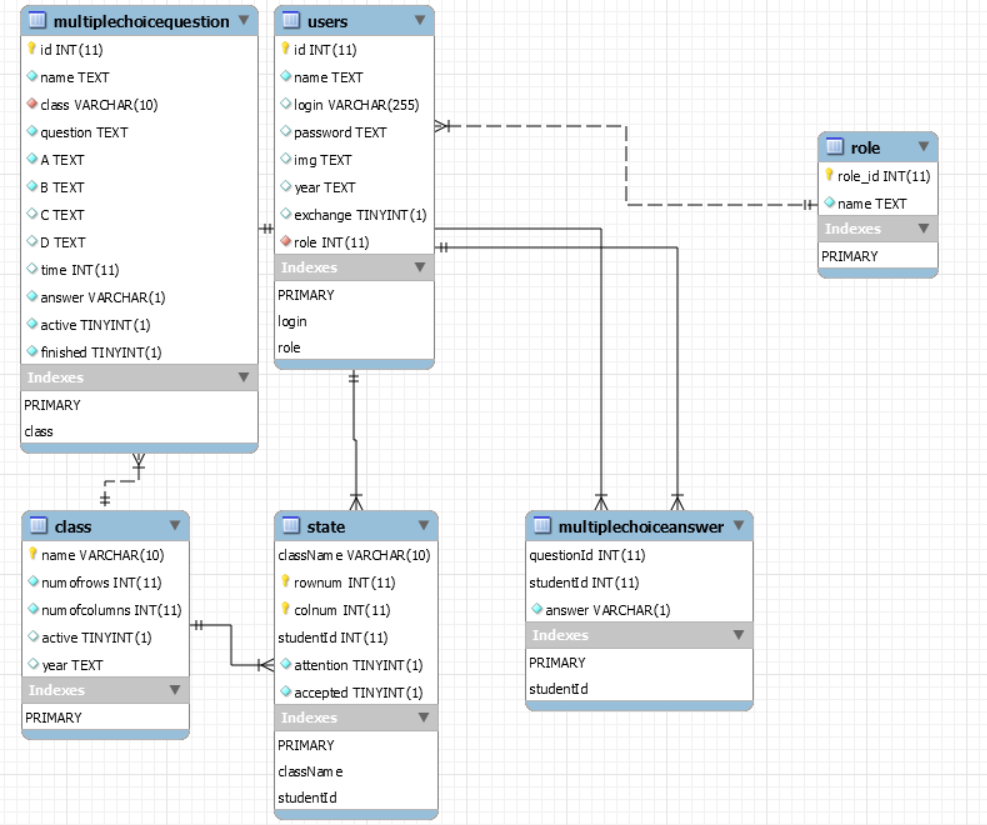
\includegraphics[width=\textwidth,height=\textheight,keepaspectratio]{images/erdiagram.png}
\end{figure}
\subsection{Class}
This entity is to represent a real life classroom. It will have a \textbf{name} as its primary key. As stated before, a class seat map is represented by a rectangle \textbf{numofrows} and \textbf{numofcolumns} are the two attributes to form that rectangle. The boolean attribute \textbf{active} is to see that if the class is active or not. The attribute \textbf{year} is to show that which intake is taking the class.

\subsection{Role}
This entity is to represent the roles that a user can have. It has an integer named \textbf{role-id} acting as the primary key, and an attributed named \textbf{name} to hold the name of the role. In my application, there are only 3 role ids for 3 roles: 1 for Administrator, 2 for Lecturer, and 3 for Student.

\subsection{Users}
This entity is to represent a user. An integer named \textbf{id} is the primary key. The attributes of this entity are \textbf{name} for the name of the user, \textbf{login} and \textbf{password} for the credentials, \textbf{img} for the path of the image of that user stored in the server, \textbf{year} is for the intake of that user (if the user is a student), \textbf{exchange} is a boolean to check that if the student is an exchange student or not, \textbf{role} is a foreign key referencing \textbf{role-id} of the table \textbf{Role}  

\subsection{State}
"State" is a concept that I created to define the connection between a student and a seat in a classroom. The primary keys are the \textbf{className}, the \textbf{rownum} and the \textbf{colnum}, which represents a seat in a classroom. \textbf{className} is also a foreign key, referencing attribute \textbf{name} of the table \textbf{Class}. The attribute \textbf{studentId}, which is a foreign key referencing the attribute \textbf{id} of table \textbf{Users}, is to represent the student sitting on the seat. The boolean attribute \textbf{attention} is to check that if that seat is calling for attention or not, and the boolean attribute \textbf{accepted} is to check that if the attention call from that seat is accepted by the lecturer or not.

\subsection{MultipleChoiceQuestion}
As stated above, in this application, a quiz is defined to consist of a single multiple choice question. \textbf{id} is its primary key, and the attribute \textbf{class}, which shows the class that that quiz belongs to, is a foreign key referencing attribute \textbf{name} of the table \textbf{Class}. The other attributes of the quiz are \textbf{name}, \textbf{question}, \textbf{A}, \textbf{B}, \textbf{C}, \textbf{D}, \textbf{time} for the time that the students have to answer the quiz, \textbf{answer} is for the solution of the quiz, \textbf{active} is a boolean to check that if that quiz is on or not, \textbf{finished} is also a boolean, and it is used to check that if that quiz is finished or not.

\subsection{MultipleChoiceAnswer}
This entity is to represent the answer of a student to the above quiz. The primary keys are \textbf{questionId} and \textbf{studentId}, which are also foreign keys that respectively referencing \textbf{id} of \textbf{MultipleChoiceQuestion}, and \textbf{id} of \textbf{Users}. The remaining attribute is \textbf{answer}, which shows the answer that a student made for a question. It could be A, B, C, D, if the student could answer the question, or N, if the student had no answer.
\section{API documentation for the back-end}

\subsection{Request}
Except for logging in, a request should always contain an Authorization header. If it is a POST or PUT request and the request body is in JSON, then there should be a Content-Type header.
\restful{
   \head{Authorization} 
        {Bearer (token)}

   \head{Content-Type} 
        {application/json}
}

\subsection{Authorization}
\subsubsection{POST /api/login}
\textbf{Request body:}
\resource{
   \attr{@login}{string}{Your username}
   \attr{@password}{string}{Your password}
}
\textbf{Response:}
\resource{
   \attr{@token}{string}{Attach this to your Authorization header for the subsequent requests}
}

\subsection{Endpoints}
\subsubsection{GET /api/showclass}
This API is to show all classrooms that are available. All roles can access this endpoint.
\textbf{Response:}
The response will be a JSON Array containing objects of classes. A class object, in this endpoint, will contain:
\resource{
   \attr{@name}{string}{Name of the classroom.}
}
Actually, the response will also show other attributes of a classroom, but they are all set to 0 or null, since for this endpoint, the only things that matters are the name of the classroom. Responses of other endpoints will also work this way; it will return all attributes of an object, but the unnecessary attributes will be set to 0 or null.

\subsubsection{POST /api/uploadFile}
This API is for the administrators to upload the image of a student to the server. Only the administrator can access this endpoint.\par
\textbf{Request parameter:}
\resource{
   \attr{@file}{file}{The image of a student}
}
\textbf{Response:}
\resource{
   \attr{@fileName}{string}{Name of the file}
   \attr{@fileDownloadUri}{string}{The path of the file in the server}
   \attr{@fileType}{string}{Type of the file}
   \attr{@size}{int}{Size of the file}
}
\subsubsection{POST /api/createclass}
This API is for the administrators to create a class. Only the administrators can access this endpoint. \par
\textbf{Request body:}
\resource{
   \attr{@name}{string}{Name of the class}
   \attr{@row}{int}{Number of rows (used to form the rectangle representing the class map)}
   \attr{@col}{int}{Number of rows (used to form the rectangle representing the class map)}
}
\subsubsection{POST /api/createstudent}
This API is for the administrators to create a student. Only the administrators can access this endpoint. \par
\textbf{Request body:}
\resource{
   \attr{@name}{string}{Name of the student}
   \attr{@img}{string}{The path of the file in the server}
   \attr{@year}{string}{The intake of the student}
   \attr{@login}{string}{The username of the student}
   \attr{@password}{string}{The password of the student}
   \attr{@exchange}{boolean}{Is this an exchange student?}
}
\subsubsection{GET /api/class}
This API is to get information of a single class. The lecturers and students can access this endpoint\par
\textbf{Request parameter:}
\resource{
   \attr{@name}{string}{Name of the class}  
}
\textbf{Response:}
\resource{
   \attr{@name}{string}{Name of the class}
   \attr{@rows}{int}{Number of rows (used to form the rectangle representing the class map)}
   \attr{@cols}{int}{Number of columns (used to form the rectangle representing the class map)}
   \attr{@active}{boolean}{Is this class active?}
   \attr{@year}{string}{The intake taking the class}
}   
\subsubsection{GET /api/state}
This API is to get the states of a class. The lecturers and students can access this endpoint\par
\textbf{Request parameter:}
\resource{
   \attr{@name}{string}{Name of the class}  
}
\textbf{Response:}
The response will be a JSON Array of state objects. A state object will look like this:
\resource{
   \attr{@row}{int}{The row-coordinate of the seat}
   \attr{@col}{int}{The column-coordinate of the seat}
   \attr{@student}{int}{The ID of the student who is taking the seat}
}
\subsubsection{GET /api/student}
This API is to get the information of a student. Only the lecturers can access this endpoint\par
\textbf{Request parameter:}
\resource{
   \attr{@id}{int}{ID of a student}  
}
\textbf{Response:}
\resource{
   \attr{@name}{string}{Name of the student}
   \attr{@img}{string}{The path of the image of that student in the server}
   \attr{@year}{string}{The intake of the student}
   \attr{@exchange}{boolean}{Is this an exchange student?}
}
\subsubsection{PUT /api/activeclass}
This API is for the lecturers to activate a class. Only the lecturers can access this endpoint\par
\textbf{Request parameter:}
\resource{
   \attr{@name}{string}{Name of the classroom}
   \attr{@year}{string}{The intake that will take that class}
}

\subsubsection{PUT /api/deactivateclass}
This API is for the lecturers to deactivate a class. Only the lecturers can access this endpoint\par
\textbf{Request parameter:}
\resource{
   \attr{@name}{string}{Name of the classroom}
}

\subsubsection{POST /api/createmultiplechoicequestion}
This API is for the lecturers to create a quiz. Only the lecturers can access this endpoint\par
\textbf{Request body:}
\resource{
   \attr{@name}{string}{Name of the quiz}
   \attr{@className}{string}{Name of the class that the quiz belongs to}
   \attr{@question}{string}{The question of the quiz}
   \attr{@A}{string}{Answer A}
   \attr{@B}{string}{Answer B}
   \attr{@C}{string}{Answer C}
   \attr{@D}{string}{Answer D}
   \attr{@time}{int}{Time allotted for the quiz}
   \attr{@solution}{string}{The character representing the right answer of the quiz}
}

\subsubsection{GET /api/average}
This API is for the lecturers to get the average result of a class on a quiz. Only the lecturers can access this endpoint. \par
\textbf{Request parameter:}
\resource{
   \attr{@questionid}{int}{ID of the quiz}
}
\textbf{Response:}
\resource{
   \attr{@right}{string}{right answers/total number of students}
   \attr{@wrong}{string}{wrong answers/total number of students}
   \attr{@no}{string}{students who had no answer/total number of students}
}

\subsubsection{GET /api/finishedquestion}
This API is for the lecturers to see the finished questions that belong to a certain class. Only the lecturers can access this endpoint. \par
\textbf{Request parameter:}
\resource{
   \attr{@className}{string}{Name of the class}
}
\textbf{Response:}
The response will be a JSON Array of quiz objects. A quiz object will look like this:
\resource{
   \attr{@id}{int}{ID of the quiz}
   \attr{@name}{string}{Name of the quiz}
}

\subsubsection{GET /api/activequestion}
This API is to show the active questions that belong to a certain class. The lecturers and students can access this endpoint. \par
\textbf{Request parameter:}
\resource{
   \attr{@className}{string}{Name of the class}
}
\textbf{Response:}
The response will be a JSON Array of quiz objects. A quiz object will look like this:
\resource{
   \attr{@id}{int}{ID of the quiz}
   \attr{@name}{string}{Name of the quiz}
}

\subsubsection{GET /api/inactivequiz}
This API is to show the inactive questions that belong to a certain class. The lecturers and students can access this endpoint. \par
\textbf{Request parameter:}
\resource{
   \attr{@className}{string}{Name of the class}
}
\textbf{Response:}
The response will be a JSON Array of quiz objects. A quiz object will look like this:
\resource{
   \attr{@id}{int}{ID of the quiz}
   \attr{@name}{string}{Name of the quiz}
}

\subsubsection{GET /api/questionname}
This API is for the lecturers to get a name of a single quiz. Only the lecturers can access this endpoint. \par
\textbf{Request parameter:}
\resource{
   \attr{@questionid}{int}{ID of the quiz}
}
\textbf{Response}
\resource{
   \attr{@name}{string}{Name of the quiz}
}

\subsubsection{POST /api/activequiz}
This API is for the lecturers to activate a quiz. Only the lecturers can access this endpoint. \par
\textbf{Request parameter:}
\resource{
   \attr{@questionid}{int}{ID of the quiz}
}

\subsubsection{GET /api/question}
This API is to show the information of a quiz. The lecturers and students can access this endpoint. \par
\textbf{Request parameter:}
\resource{
   \attr{@questionid}{int}{ID of the quiz}
}
\textbf{Response:}
\resource{
   \attr{@name}{string}{Name of the quiz}
   \attr{@className}{string}{Name of the class that the quiz belongs to}
   \attr{@question}{string}{The question of the quiz}
   \attr{@A}{string}{Answer A}
   \attr{@B}{string}{Answer B}
   \attr{@C}{string}{Answer C}
   \attr{@D}{string}{Answer D}
   \attr{@time}{int}{Time allotted for the quiz}
   \attr{@solution}{string}{The character representing the right answer of the quiz}
}

\subsubsection{GET /api/quiztime}
This API is to show the remaining time of a quiz. The lecturers and students can access this endpoint. \par
\textbf{Request parameter:}
\resource{
   \attr{@questionid}{int}{ID of the quiz}
}
\textbf{Response:}
\resource{
   \attr{@time}{int}{The remaining time of the quiz}
}

\subsubsection{GET /api/quizreview}
This API is to the information of a quiz, and the result of a particular student on that quiz. The lecturers and students can access this endpoint. \par
\textbf{Request parameter:}
\resource{
   \attr{@questionid}{int}{ID of the quiz}
   \attr{@studentid}{int}{ID of the student}
}
\textbf{Response:}
\resource{
   \attr{@name}{string}{Name of the quiz}
   \attr{@question}{string}{The question of the quiz}
   \attr{@A}{string}{Answer A}
   \attr{@B}{string}{Answer B}
   \attr{@C}{string}{Answer C}
   \attr{@D}{string}{Answer D}
   \attr{@solution}{string}{The character representing the right answer of the quiz}
}
\subsubsection{GET /api/answerbyseat}
This API is for the lecturers to see the answers of the student by seats. Only the lecturers can access this endpoint. \par
\textbf{Request parameter:}
\resource{
   \attr{@questionid}{int}{ID of the quiz}
}
\textbf{Response:}
The response will be a JSON Array containing objects of AnswerBySeat. An AnswerBySeat object, in this endpoint, will contain:
\resource{
   \attr{@name}{string}{Name of the student}
   \attr{@img}{string}{The path for the image of that student in the server}
   \attr{@row}{int}{The row-coordinate of the seat that that student is sitting in}
   \attr{@col}{int}{The column-coordinate of the seat that that student is sitting in}
   \attr{@answer}{string}{The answer of that student}
   \attr{@solution}{string}{The solution of the quiz}
}

\subsubsection{PUT /api/callattention}
This API is for the students to call for attention. Only the students can access this endpoint. \par
\textbf{Request parameter:}
\resource{
   \attr{@studentid}{int}{ID of the student}
}

\subsubsection{PUT /api/closeattention}
This API is to close the call for attention. The lecturers and students can access this endpoint. \par

\subsubsection{GET /api/checkattention}
This API is for the lecturers to check if any student is calling for attention or not. Only the lecturers can access this endpoint. \par
\textbf{Request parameter:}
\resource{
   \attr{@classname}{int}{Name of the class}
} 
\textbf{Response:}
\resource{
   \attr{@row}{int}{Row-coordinate of the student who is calling for attention}
   \attr{@col}{int}{Column-coordinate of the student who is calling for attention}
   \attr{@studentId}{int}{ID of the student who is calling for attention}
}

\subsubsection{PUT /api/setaccepted}
This API is to modify the state of acceptance for a call for attention. The lecturers and students can access this endpoint. \par
\textbf{Request parameter:}
\resource{
   \attr{@turn}{string}{Only two values are allowed: "on" or "off". "On" means that the call is accepted, "off" means that the call is done and not accepted anymore}
} 

\subsubsection{POST /api/createstate}
This API is for the students to create states. Only the students can access this endpoint. \par
\textbf{Request body:}
\resource{
   \attr{@class}{string}{The name of the class}
   \attr{@row}{int}{Row-coordinate of the seat that that student wants to sit in}
   \attr{@col}{int}{Column-coordinate of the seat that that student wants to sit in}
   \attr{@student}{int}{ID of the student}
}

\textbf{Response:}
\resource{
   \attr{@Result}{string}{Result of the state creation process.}
} 
\subsubsection{POST /api/createmultiplechoiceanswer}
This API is for the students to create an answer for a quiz. Only the students can access this endpoint. \par
\textbf{Request body:}
\resource{
   \attr{@questionId}{int}{The id of the quiz}
   \attr{@studentId}{int}{The id of the student}
   \attr{@answer}{string}{The character representing the answer of the student}
}

\subsubsection{GET /api/quizdone}
This API is to show the quizzes done by a student. Only the students can access this endpoint.  \par
\textbf{Request parameter:}
\resource{
   \attr{@studentid}{int}{ID of the student}
}
\textbf{Response:}
The response will be a JSON Array of quiz objects. A quiz object will look like this:
\resource{
   \attr{@id}{int}{ID of the quiz}
   \attr{@name}{string}{Name of the quiz}
}

\subsubsection{GET /api/checkaccepted}
This API is for a student to check that if their call for attention is accepted or not. Only the students can access this endpoint.  \par
\textbf{Request parameter:}
\resource{
   \attr{@studentid}{int}{ID of the student}
}
\textbf{Response:}
\resource{
   \attr{@Result}{boolean}{Is the call for attention accepted?}
}
\chapter{Conclusion}
\printbibliography[title = References]
\addcontentsline{toc}{chapter}{References}
\end{document}
